\documentclass[UTF8,a4paper,12pt]{ctexart}
\usepackage[a4paper,top=2.45cm,bottom=2.45cm,left=2.55cm,right=2.55cm]{geometry}
\usepackage{amsmath,amssymb,bm,graphicx,booktabs,array,multirow,longtable,siunitx,float,caption,subcaption,enumitem,xcolor,fancyhdr,hyperref}
\graphicspath{{report/figures/}{figures/}}
\sisetup{detect-all,per-mode=symbol,range-phrase=--,range-units=single}
\setlength{\parindent}{2em}
\setlength{\parskip}{0.25em}
\setlist{itemsep=0.2em,topsep=0.3em}
\captionsetup{font=small,labelfont=bf}
\hypersetup{colorlinks=true,linkcolor=blue!50!black,citecolor=blue!50!black,urlcolor=blue!50!black}
\newcolumntype{L}[1]{>{\raggedright\arraybackslash}p{#1}}
\newcommand{\DOE}{\mathrm{DOE}}
\newcommand{\um}{\si{\micro\meter}}
\newcommand{\mm}{\si{\milli\meter}}
\pagestyle{fancy}
\setlength{\headheight}{15pt}
\fancyhf{}
\fancyhead[L]{共享高度 DOE 的多波长像面重建}
\fancyhead[R]{数值研究报告}
\fancyfoot[C]{\thepage}

\title{\heiti 基于共享物理高度 DOE 的多波长像面衍射图案重建与 RGB 消色散数值研究}
\author{姓名：\underline{\hspace{4cm}}\\学号：\underline{\hspace{4cm}}\\课程班级：\underline{\hspace{4cm}}\\指导教师：\underline{\hspace{4cm}}}
\date{2026年10月5日}

\begin{document}
\maketitle
\thispagestyle{empty}

\begin{abstract}
本研究围绕一个具体而具有代表性的衍射光学问题展开：同一张具有共享物理高度图的静态衍射光学元件（diffractive optical element, DOE），能否在多个波长下，于同一个物理像面形成位置一致、形状相近且背景可接受的目标图案。研究采用标量角谱传播模型，以 Shipley S1813 光刻胶的色散折射率为材料模型，设计波长覆盖 \SI{488}{nm}、\SI{532}{nm} 和 \SI{633}{nm}。在研究过程中，先后完成了双圆斑和双圆环的双波长优化、包括方形和十字在内的 RGB 多图案泛化比较、角谱 FFT 与小网格稠密传播矩阵的可信度验证，以及 RGB 跨波长一致性损失的正式消融实验。

结果表明，正确的物理采样、孔径覆盖检查和共同色标评价对于判断所谓“颜色差异”十分关键。双波长阶段可以得到清晰的双圆斑和空心圆环，但圆环的跨波长位置漂移显著大于圆斑。RGB 泛化实验显示，十字和较大半径圆环相对容易重建，而小圆环、圆斑和含尖角图案仍受边缘质量、背景和跨波长位置的共同限制。正式完成的 $7$ 种损失变体、$3$ 类目标、$2$ 种光路和 $3$ 个随机种子的共 $126$ 次实验表明，加入逐像素跨波长一致性和绝对能量一致性后，六个目标--光路单元的共同尺度 ROI Pearson 相关系数均显著提高，RGB ROI 能量变异系数也明显下降；但多数单元的背景比例同步升高。因此，本研究支持“在有限目标集合和当前数值模型下可以获得部分 RGB 像素级消色散改进”，但不支持“任意图案均可无代价消色散”的更强结论。全文同时明确区分了数值模拟已经验证的内容与尚未涉及的加工、测量和真实光学系统问题。
\end{abstract}

\noindent\textbf{关键词：} 衍射光学元件；多波长 DOE；角谱传播；RGB 消色散；像面重建；共享高度优化
\tableofcontents
\newpage

\section{研究背景与问题定义}
\subsection{研究问题}
传统静态 DOE 的相位延迟由物理高度和材料折射率共同决定。对于单一设计波长，优化一张高度图以形成两个光斑、一个环形结构或一个非圆形轮廓通常是可行的；然而，当入射光包含多个波长时，相同高度在不同波长下产生的相位延迟不同，且衍射传播本身也具有波长依赖性。因此，单波长上表现良好的 DOE，换到 RGB 光源后可能出现光斑横向平移、轮廓宽度改变、环半径变化、彩色边缘和背景噪声。

本课题将“相同衍射图案”定义为：不同波长的像面强度在同一物理坐标系中具有相近的目标几何位置和空间结构，而不是仅仅具有相同的衍射级次或相同的角度方向。具体而言，评价同时包含四个层次：
\begin{enumerate}
\item \textbf{形状重建：} 输出强度与目标强度的相关系数、振幅误差和强度误差；
\item \textbf{空间位置：} 各光斑或圆环组件的质心误差以及 RGB 间质心漂移；
\item \textbf{能量分配：} ROI 效率、背景比例和各组件能量平衡；
\item \textbf{跨波长一致性：} 共同线性色标下的逐像素相似度、边缘一致性、背景一致性和绝对能量变异。
\end{enumerate}
所有目标均独立优化，不要求同一张 DOE 同时产生多种不同图案。这里的“泛化性”指一种优化方法面对不同目标形状时，能否保持稳定的重建质量，而不是把一张已经优化好的 DOE 直接迁移到另一目标上。

\subsection{研究动机与相关工作}
多波长 DOE 的核心困难并非简单地把单波长实验重复几次，而是不同波长必须共享同一物理高度自由度。Kim、Domínguez-Caballero 和 Menon 对多波长衍射光学的高度优化、离散搜索以及高度误差进行了系统研究\cite{kim2012}；Chen 等人直接讨论了多色 LED 获得相同衍射图案的问题\cite{chen2016}。Bowman 等人的多波长全息研究则代表了另一类可编程空间光调制器路线\cite{bowman2015}。这些工作共同说明，多波长图案一致性必须作为设计目标处理，而不能仅通过显示阶段的通道归一化来掩盖。

本项目选择静态共享高度 DOE，而不是逐波长独立的相位板或实时 SLM。这样做的优点是物理问题明确、器件结构简单；代价是所有波长共用同一张高度图，优化自由度受到严格限制。研究的目标不是证明任意图案都能在任意光学系统中被完美消色散，而是建立一套可以逐层验证的数值流程，并用多类目标和多种指标回答：哪些图案容易实现，哪些指标会冲突，以及增加跨波长损失是否真的改善了像素级一致性。

\subsection{研究边界}
本报告中的结论均属于理想标量传播条件下的数值结论。研究没有把模拟结果直接等同于已加工器件的实测性能，也没有将 CIE 色度学、真实激光功率谱、探测器响应、偏振、吸收、反射、表面粗糙度和全波电磁效应纳入主模型。后文会把已经完成的工作和明确没有完成的工作分开列出。

\section{物理模型与数值方法}
\subsection{共享物理高度 DOE}
设 DOE 的物理高度为 $h(x,y)$，入射孔径振幅为 $A(x,y)$，空气折射率取 $n_{\mathrm{air}}=1$。在波长 $\lambda$ 下，DOE 后的复振幅写为
\begin{equation}
U_{\lambda}^{\mathrm{DOE}}(x,y)=A(x,y)\exp\left[\mathrm{i}\,\phi_{\lambda}(x,y)\right],\qquad
\phi_{\lambda}(x,y)=\frac{2\pi\left[n(\lambda)-n_{\mathrm{air}}\right]}{\lambda}h(x,y).
\label{eq:doe-phase}
\end{equation}
关键约束是所有波长使用同一个 $h(x,y)$，而 $n(\lambda)$ 和 $\lambda$ 进入相位关系。该表达式没有给每个波长单独分配一张相位图，因此保留了静态器件的实际物理限制。

\subsection{角谱传播与 FFT 坐标约定}
自由传播采用角谱法。对于传播距离 $z$，有
\begin{equation}
U_{\lambda}(x,y;z)=\mathcal{F}^{-1}\left\{\mathcal{F}\left[U_{\lambda}^{\mathrm{DOE}}(x,y)\right]H_{\lambda}(f_x,f_y;z)\right\}.
\label{eq:angular-spectrum}
\end{equation}
其中传递函数的传播分量写为
\begin{equation}
H_{\lambda}(f_x,f_y;z)=\exp\left[\mathrm{i}2\pi z\sqrt{\lambda^{-2}-f_x^2-f_y^2}\right].
\end{equation}
FFT 的顺序固定为“居中物理场、\texttt{ifftshift}、FFT、乘角谱传递函数、IFFT、\texttt{fftshift}、居中输出场”。零距离恒等测试、能量测试和稠密矩阵复现测试均针对这一具体约定进行，而不是仅验证抽象的傅里叶变换公式。

\subsection{S1813 色散模型}
材料折射率采用二项 Cauchy 模型
\begin{equation}
n(\lambda)=A+\frac{B}{\lambda^2},\qquad A=1.60222794799,\quad B=1.30111940487\times10^{-14}\,\mathrm{m^2}.
\label{eq:cauchy}
\end{equation}
\SI{532}{nm} 和 \SI{633}{nm} 的折射率作为文献锚点，\SI{488}{nm} 则由模型外推。

\begin{table}[H]
\centering
\caption{S1813 折射率取值及来源。}
\label{tab:refractive-index}
\begin{tabular}{cccc}
\toprule
波长 / \si{nm} & $n(\lambda)$ & 来源 & 是否外推 \\
\midrule
488 & 1.656864 & Cauchy 模型外推 & 是 \\
532 & 1.648200 & Kim 等文献锚点 & 否 \\
633 & 1.634700 & Kim 等文献锚点 & 否 \\
\bottomrule
\end{tabular}
\end{table}
因此，报告中的 RGB 结果不能把 \SI{488}{nm} 的折射率表述为直接测量值。$\Delta n=\pm0.005$ 的检查属于后验敏感性分析，不等同于使用实测色散曲线重新训练后的鲁棒性证明。

\subsection{采样、孔径和两种光路}
正式优化使用正确覆盖 \SI{1}{mm} 半径 DOE 孔径的粗到细采样。粗阶段和精阶段的物理视场均为 \SI{2.56}{mm}，孔径直径为 \SI{2.00}{mm}，视场与孔径直径之比为 $1.28$，超过预设的 $1.2$ 下限。零填充因子为 $2$。
\begin{table}[H]
\centering
\caption{正式优化的采样设置。}
\label{tab:sampling}
\begin{tabular}{cccc}
\toprule
阶段 & 网格 & 像素间距 / \si{\micro\meter} & 物理视场 / \si{mm} \\
\midrule
粗优化 & $256\times256$ & 10 & 2.56 \\
精优化 & $512\times512$ & 5 & 2.56 \\
\bottomrule
\end{tabular}
\end{table}

主实验比较两种光路：\textbf{单 DOE} 为 DOE 后自由传播 \SI{50}{mm} 到像面；\textbf{双 DOE} 为 DOE1 自由传播 \SI{25}{mm} 到 DOE2，再传播 \SI{25}{mm} 到像面。两种光路使用相同材料模型、孔径、波长、目标和评价接口。此前测试过的 \texttt{doe\_fourier\_lens} 由于共同色标下色散明显，被保留为历史对照，但不进入后续 RGB 消融主结论。

\subsection{优化方法}
连续高度优化以 Adam 为主，并保留一种 Adam 中加入背景混合/偏置风格项的 MRAF 风格路线。本文中的 MRAF 不是独立的经典 MRAF/GS 迭代投影算法，而是对现有梯度优化过程的背景自由度修正。早期双波长阶段还使用过 64 级 DBS 作为算法对照，但其在多目标和长迭代实验中表现不稳定，后续 RGB 消色散主实验不再纳入 DBS。

\section{目标图案与评价指标}
\subsection{目标图案演化}
目标设计经历了由简单到复杂的三阶段。第一阶段以横向双软边圆斑和双圆环为主，圆斑半径约 \SI{40}{\micro\meter}，圆环优先使用外半径 \SI{50}{\micro\meter}、宽度 \SI{8}{\micro\meter}，另对 \SI{60}{\micro\meter} 圆环进行比较。第二阶段扩展到八类 RGB 目标：双软边圆斑、$R=50\,\um$ 双圆环、$R=60\,\um$ 双圆环、双方形、双十字、三角形三圆斑、实心三角形和左右不对称双圆斑。第三阶段为了集中判断消色散损失的作用，固定为双圆斑、双十字和 $R=50\,\um$ 双圆环三类目标。

多光斑目标均保存独立 component mask；连续几何目标则保存 signal、transition 和 background mask。目标强度非负并归一化，但在 RGB 绝对能量评价中不把每个波长的像面强度再次归一化为总和 $1$，以免隐藏真实的通道功率差。

\begin{table}[H]
\centering
\caption{研究中使用的主要目标及其困难来源。}
\label{tab:targets}
\resizebox{\textwidth}{!}{%
\begin{tabular}{L{3.0cm}L{6.2cm}L{5.0cm}}
\toprule
目标 & 几何定义 & 主要评价重点 \\
\midrule
双软边圆斑 & 两个中心约为 $(-300,0)$ 和 $(300,0)\,\um$ 的有限半径圆斑 & 相关系数、质心误差、左右能量平衡 \\
双圆环 & 两个相同半径和宽度的圆环，优先比较 $R=50$ 和 $60\,\um$ & 中心/环带比、内孔泄漏、环半径误差、跨波长漂移 \\
双方形 & 边长约 $80\,\um$、软化宽度 $15\,\um$ 的两个方形 & 四边位置、四角保持率、边缘粗糙度 \\
双十字 & 水平臂和垂直臂长度约 $80\,\um$、臂宽约 $20\,\um$ & 臂长、臂宽、交叉中心、端部衰减 \\
三角形三圆斑 & $(-300,0)$、$(300,0)$、$(0,300)\,\um$ 三个半径 $40\,\um$ 的圆斑 & 三组件能量、质心、三角形布局误差 \\
实心三角形 & 外接圆半径约 $60\,\um$、顶点朝上的软边等边三角形 & 三条边、顶点位置、角点钝化、内部效率 \\
不对称双圆斑 & 左右强度目标比例约 $1:0.65$ & 目标能量比例、组件质心和独立相关性 \\
\bottomrule
\end{tabular}}
\end{table}

\subsection{通用像面指标}
设目标信号区为 $S$、过渡区为 $T$、背景区为 $B$，输出强度为 $I_\lambda$，则基础评价包括
\begin{align}
C_\lambda &= \operatorname{corr}\left(I_\lambda|_S,I_{\mathrm{target}}|_S\right),\\
E_{\mathrm{ROI},\lambda} &= \frac{\sum_{(x,y)\in S}I_\lambda(x,y)}{\sum_{x,y}I_\lambda(x,y)+\epsilon},\\
B_\lambda &= \frac{\sum_{(x,y)\in B}I_\lambda(x,y)}{\sum_{x,y}I_\lambda(x,y)+\epsilon}.
\end{align}
同时记录振幅 MSE、强度 MSE、每个组件的质心误差、FWHM、圆形度和峰值/平均背景对比度。圆环再记录中心/环带强度比、环峰半径、半径误差和内孔泄漏。

\subsection{RGB 共同色标指标}
对于跨波长比较，先使用共同线性色标
\begin{equation}
I_{\max}=\max_{\lambda,x,y}I_\lambda(x,y),
\end{equation}
而不是逐波长峰值归一化。另设形状归一化版本，用于只观察空间结构。共同尺度 ROI Pearson 反映 RGB 像素级空间相似度，RGB ROI 能量变异系数定义为
\begin{equation}
\mathrm{CV}_{\mathrm{RGB}}=
\frac{\operatorname{std}(\eta_{488},\eta_{532},\eta_{633})}
{\operatorname{mean}(\eta_{488},\eta_{532},\eta_{633})+\epsilon},
\end{equation}
其中 $\eta_\lambda$ 是输入能量归一化后的 ROI 绝对效率。该指标与形状 Pearson 必须同时报告，因为“形状一致但能量不同”和“能量平衡但纹理不同”是两类不同的结果。

\section{传播模型可信度验证}
\subsection{小网格稠密传播矩阵}
为判断颜色差异究竟来自物理传播还是来自实现错误，构造了 $N^2\times N^2$ 的角谱稠密矩阵和离散 Fresnel 核矩阵。验证网格为 $16$、$24$、$32$、$48$、$64$，物理视场固定为 $320\,\um\times320\,\um$，传播距离为 \SI{10}{mm}，孔径半径为 \SI{120}{\micro\meter}。单矩阵显存上限为 \SI{256}{MiB}，实际最大的 $64\times64$ 角谱矩阵约占 \SI{128}{MiB}。

\begin{figure}[H]
\centering
\begin{subfigure}{0.48\textwidth}
  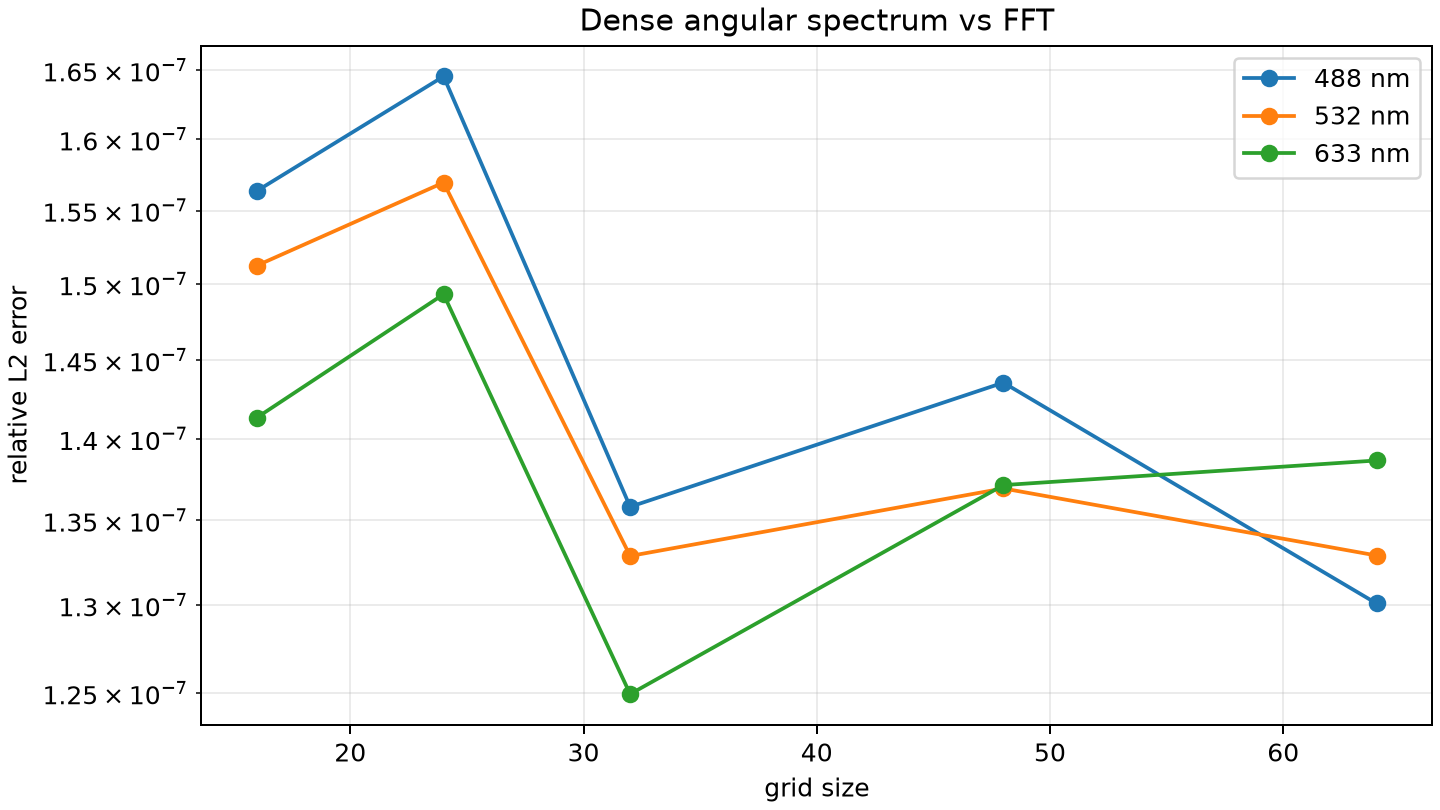
\includegraphics[width=\linewidth]{prop_angular_dense_vs_fft_error.png}
  \caption{角谱稠密矩阵与 FFT。}
\end{subfigure}\hfill
\begin{subfigure}{0.48\textwidth}
  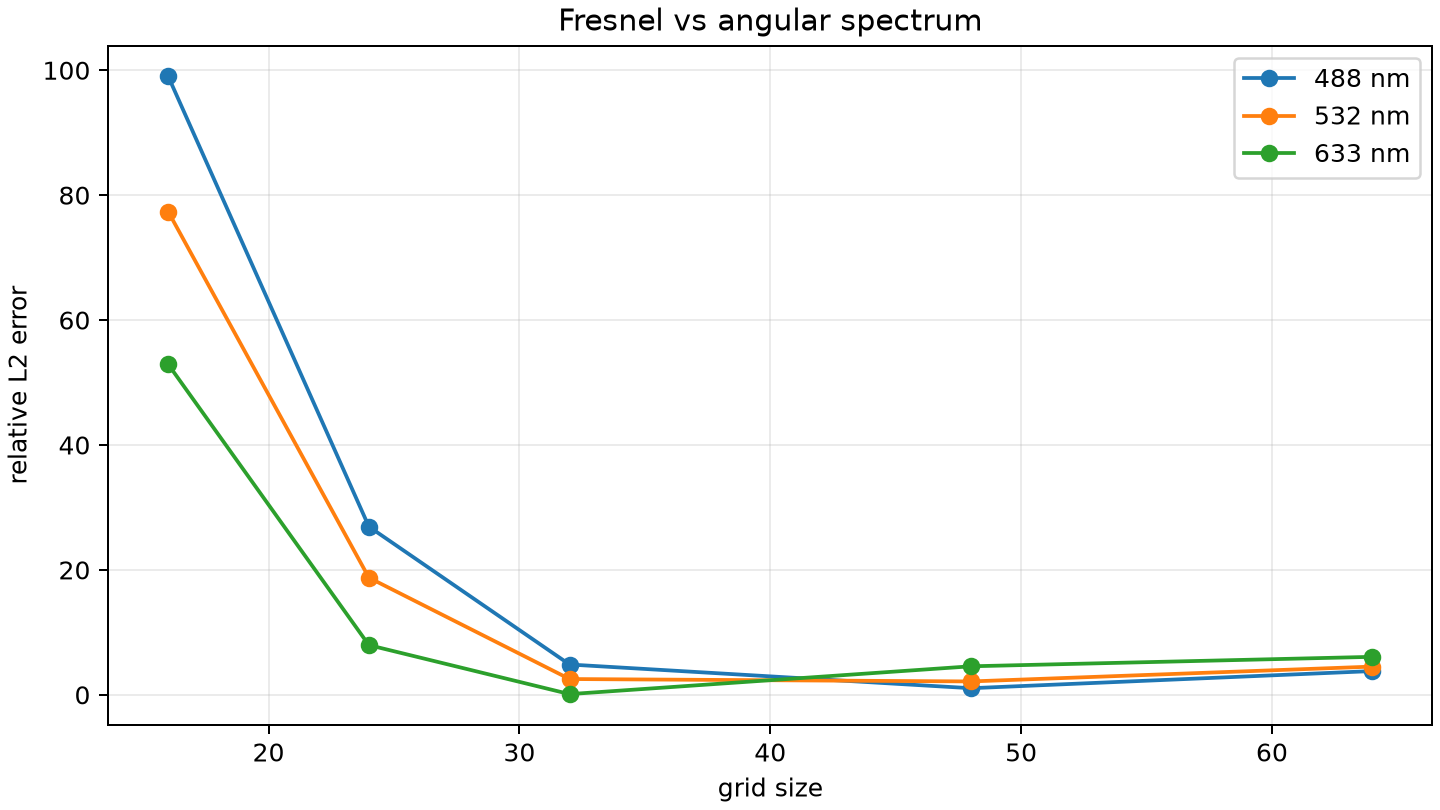
\includegraphics[width=\linewidth]{prop_fresnel_vs_angular_error.png}
  \caption{Fresnel 与角谱。}
\end{subfigure}
\caption{小网格传播算子的一致性与近似差异。角谱稠密矩阵复现 FFT，而 Fresnel 矩阵反映的是另一种离散近似。}
\label{fig:propagation-errors}
\end{figure}

角谱稠密矩阵与 FFT 的最大相对 L2 误差为 $1.65\times10^{-7}$，低于 $10^{-5}$ 验收阈值；所有矩阵均为有限数值。传播能量相对误差最大为 $5.36\times10^{-7}$，处于当前浮点和离散实现的数值误差范围。相比之下，Fresnel 与角谱的差异并不单调地随网格增大而下降：$16\times16$ 时平均差异约为 $0.764$，$32\times32$ 时下降到约 $0.025$，$64\times64$ 又约为 $0.048$。这说明 Fresnel 结果不能直接当作角谱 FFT 的等价替代，坐标、边界和离散归一化仍会影响有限网格结果。

\begin{table}[H]
\centering
\caption{传播验证按网格汇总的主要误差。Fresnel 列为三个波长的平均相对 L2 误差。}
\label{tab:propagation-summary}
\begin{tabular}{ccccc}
\toprule
网格 & 角谱稠密--FFT 最大误差 & Fresnel--角谱平均误差 & 能量误差最大值 & 矩阵显存 \\
\midrule
16 & $1.56\times10^{-7}$ & 0.764 & $5.36\times10^{-7}$ & 0.5 MiB \\
24 & $1.65\times10^{-7}$ & 0.179 & $1.79\times10^{-7}$ & 2.53 MiB \\
32 & $1.36\times10^{-7}$ & 0.025 & $2.98\times10^{-7}$ & 8.0 MiB \\
48 & $1.44\times10^{-7}$ & 0.026 & $2.38\times10^{-7}$ & 40.5 MiB \\
64 & $1.39\times10^{-7}$ & 0.048 & $2.98\times10^{-7}$ & 128 MiB \\
\bottomrule
\end{tabular}
\end{table}

\subsection{坐标与衍射级次检查}
固定相位光栅的理论一级位置为
\begin{equation}
x_{\pm1}=\pm\frac{\lambda z}{p},
\end{equation}
其中 $p$ 为光栅周期。实际像面中各级次质心与理论位置总体一致，误差大多受像素化和零填充影响。在 $64\times64$、\SI{633}{nm} 的边界案例中，一级位置误差约为 \SI{10.007}{\micro\meter}，比按 $\max(2\Delta x,0.05|x_{\mathrm{theory}}|)$ 计算的 \SI{10}{\micro\meter} 阈值高出约 \SI{0.007}{\micro\meter}，应理解为临界数值案例，而不是明显的坐标错误。

\begin{figure}[H]
\centering
\begin{subfigure}{0.48\textwidth}
  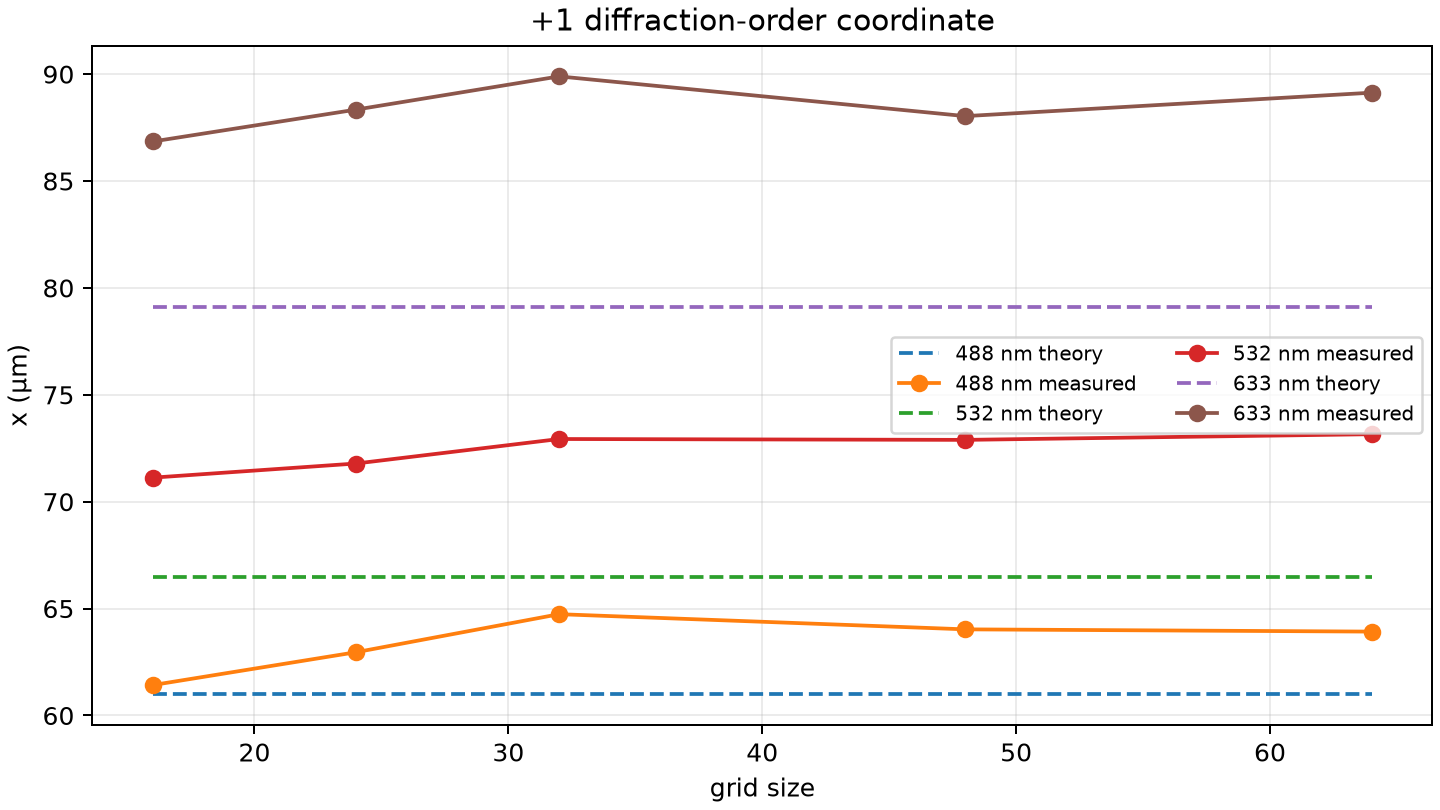
\includegraphics[width=\linewidth]{prop_diffraction_order_position.png}
  \caption{理论与实际级次位置。}
\end{subfigure}\hfill
\begin{subfigure}{0.48\textwidth}
  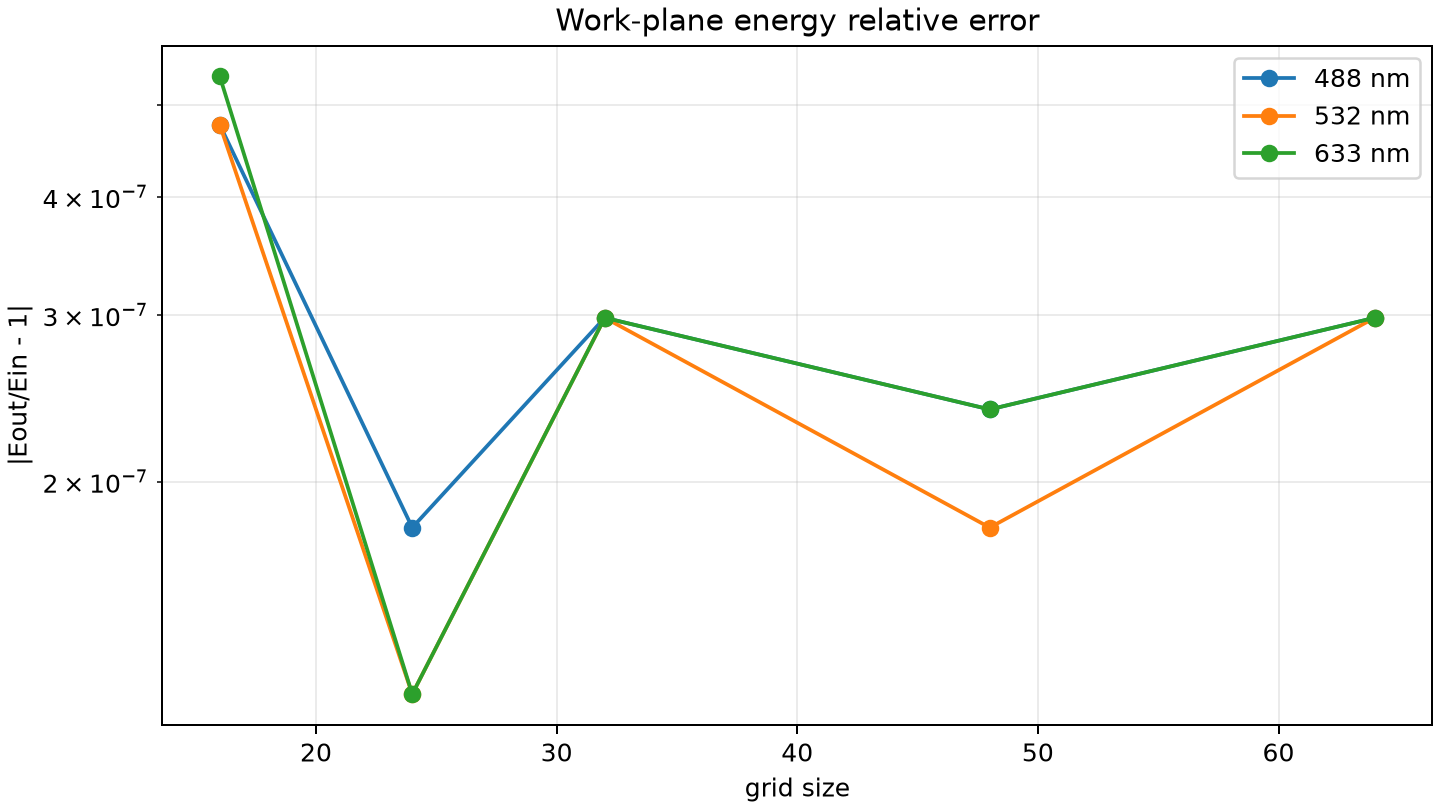
\includegraphics[width=\linewidth]{prop_energy_conservation.png}
  \caption{能量相对误差。}
\end{subfigure}
\caption{传播坐标和能量守恒检查。}
\label{fig:propagation-checks}
\end{figure}

\subsection{对正式 DOE 模型的意义}
真实 DOE 模型的 $256\times256$、\SI{10}{\micro\meter} 和 $512\times512$、\SI{5}{\micro\meter} 两种设置均通过孔径完整覆盖检查，视场/孔径直径比均为 $1.28$。这一步排除了早期“\SI{256}{\micro\meter} 网格、\SI{5}{\micro\meter} 像素却试图容纳 \SI{1}{mm} 半径孔径”的不一致设置。稠密矩阵验证说明当前 FFT 的传播坐标实现可信，但不意味着稠密矩阵适合直接替代大网格 FFT；其存储和乘法代价随 $N^4$ 增长，实际用途限于小网格算子核验和可控模型研究。

\section{双波长圆斑与圆环结果}
\subsection{双圆斑}
第一阶段以 \SI{532}{nm} 和 \SI{633}{nm} 为设计波长，采用粗网格预优化、细网格继承和 Adam/MRAF 风格精修。正式阶段报告中，双圆斑的最差波长相关系数约为 $0.924$--$0.929$，背景比例约为 $2\%$--$3\%$，跨波长质心漂移约为 \SI{4}{\micro\meter}。这说明对圆斑而言，目标本身的边界平滑、光斑尺寸和较宽的频谱容忍度有利于共享高度优化。

\begin{figure}[H]
\centering
\begin{subfigure}{0.31\textwidth}
  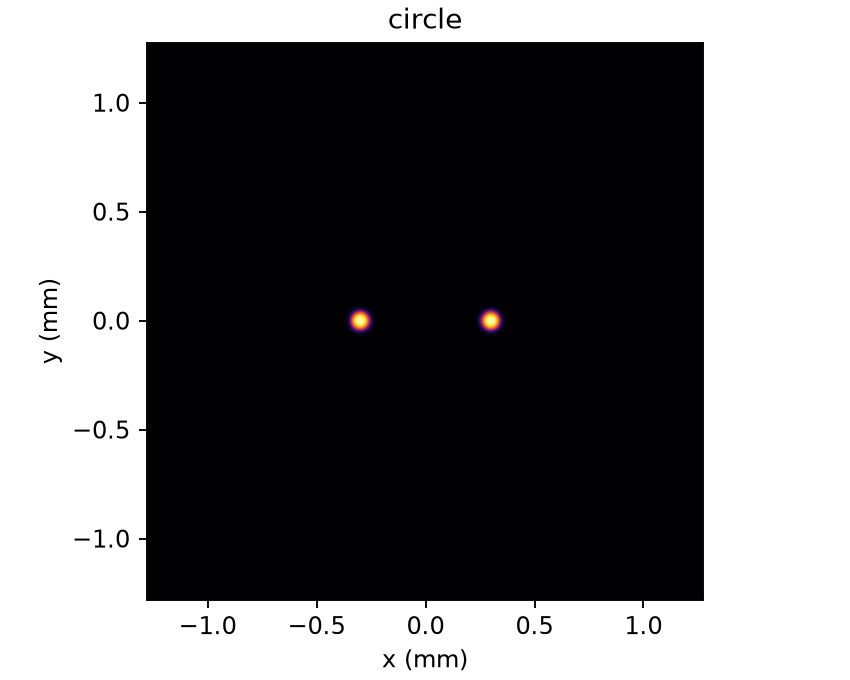
\includegraphics[width=\linewidth]{ring_circle_target.png}
  \caption{目标。}
\end{subfigure}\hfill
\begin{subfigure}{0.31\textwidth}
  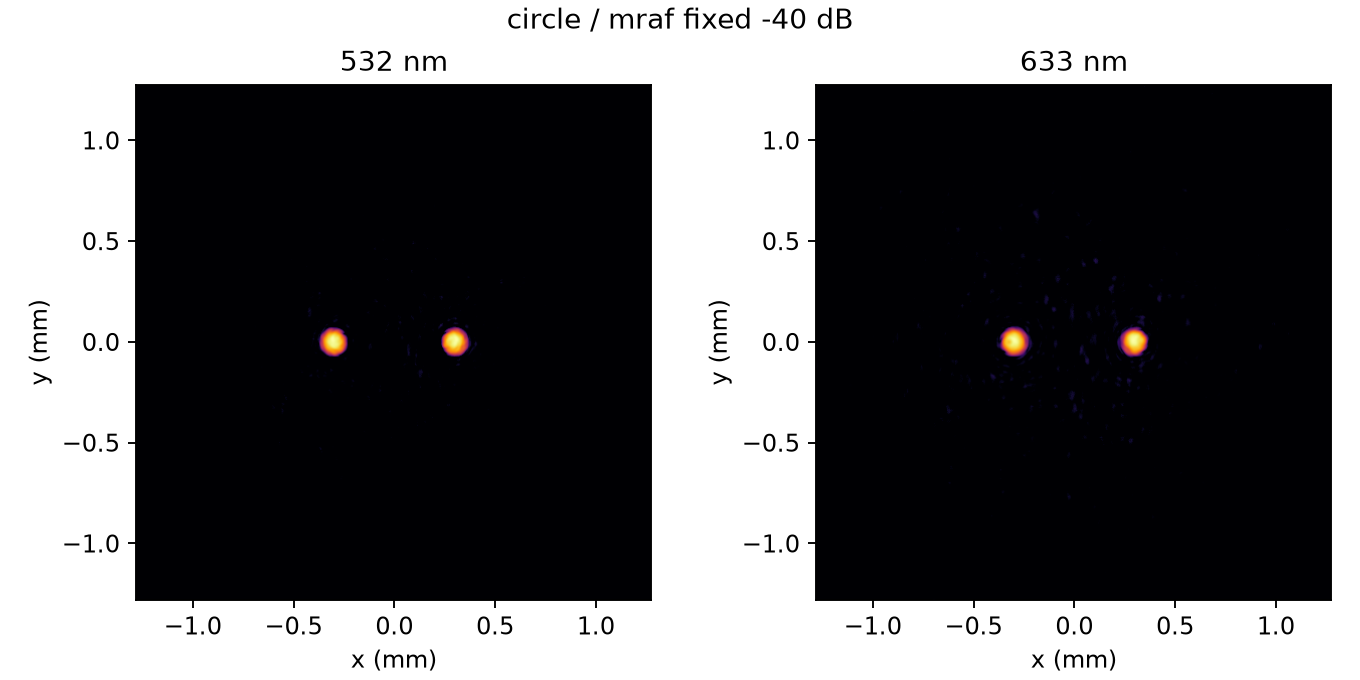
\includegraphics[width=\linewidth]{ring_circle_output.png}
  \caption{像面输出。}
\end{subfigure}\hfill
\begin{subfigure}{0.31\textwidth}
  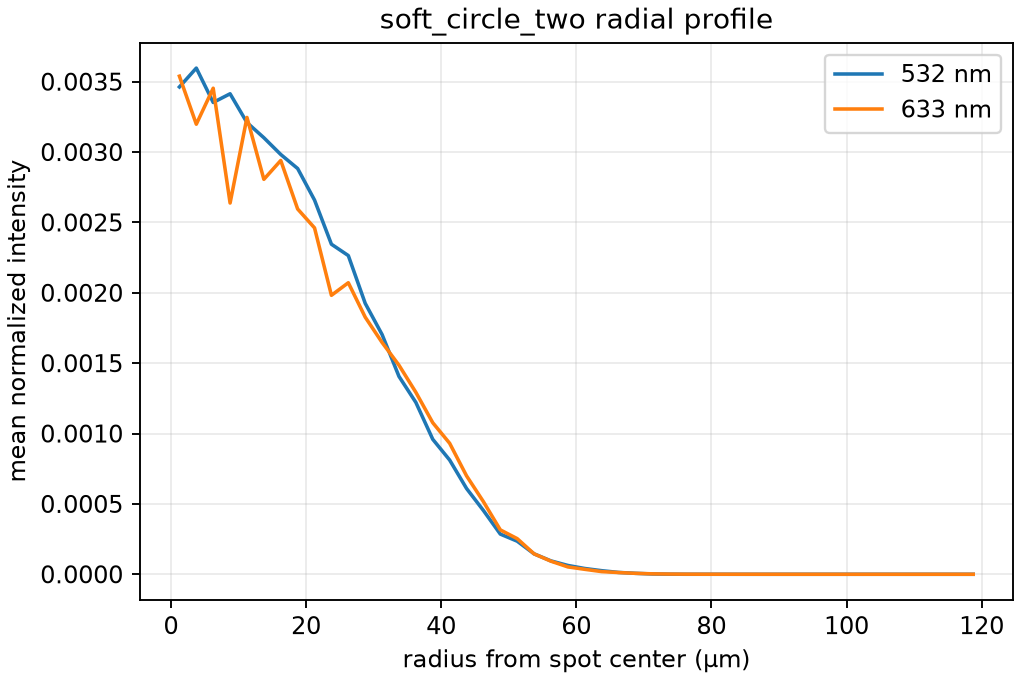
\includegraphics[width=\linewidth]{ring_circle_profile.png}
  \caption{径向剖面。}
\end{subfigure}
\caption{双圆斑阶段的代表性像面结果。输出图为固定负四十 dB 显示范围的像面强度图，不是 DOE 高度图。}
\label{fig:two-spots}
\end{figure}

\subsection{双圆环}
圆环是本课题中更能暴露问题的目标。$R=50\,\um$ 和 $R=60\,\um$ 的环形信号需要同时满足“环带有能量”和“中心保持空洞”两个相互制约的条件。第一阶段结果显示，圆环相关系数约为 $0.80$--$0.83$，中心/环带强度比约为 $0.002$--$0.003$，空心结构本身清晰；但不同波长的环中心漂移约为 \SIrange{29}{36}{\micro\meter}，明显大于双圆斑。

\begin{figure}[H]
\centering
\begin{subfigure}{0.31\textwidth}
  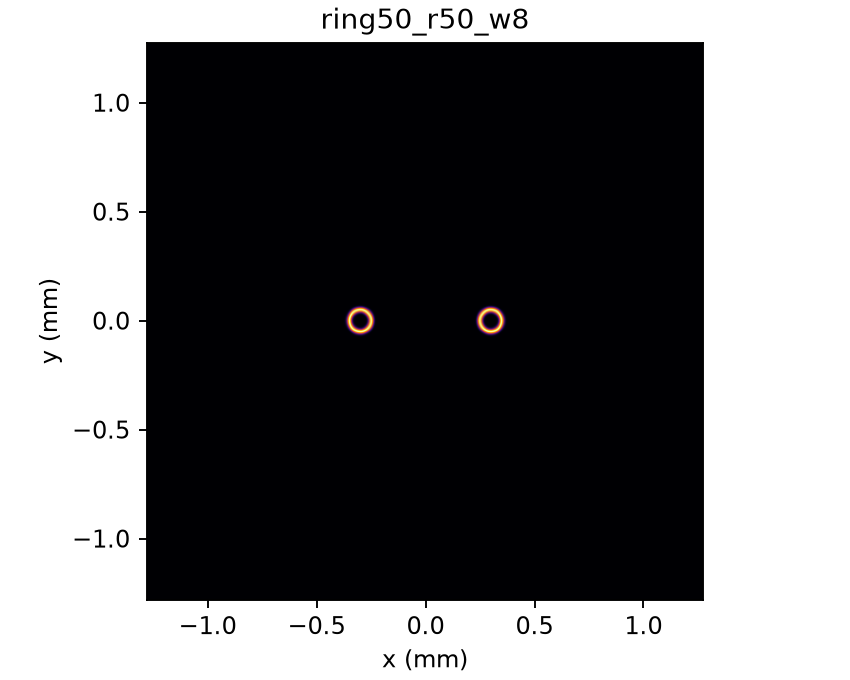
\includegraphics[width=\linewidth]{ring50_target.png}
  \caption{$R=50\,\um$ 目标。}
\end{subfigure}\hfill
\begin{subfigure}{0.31\textwidth}
  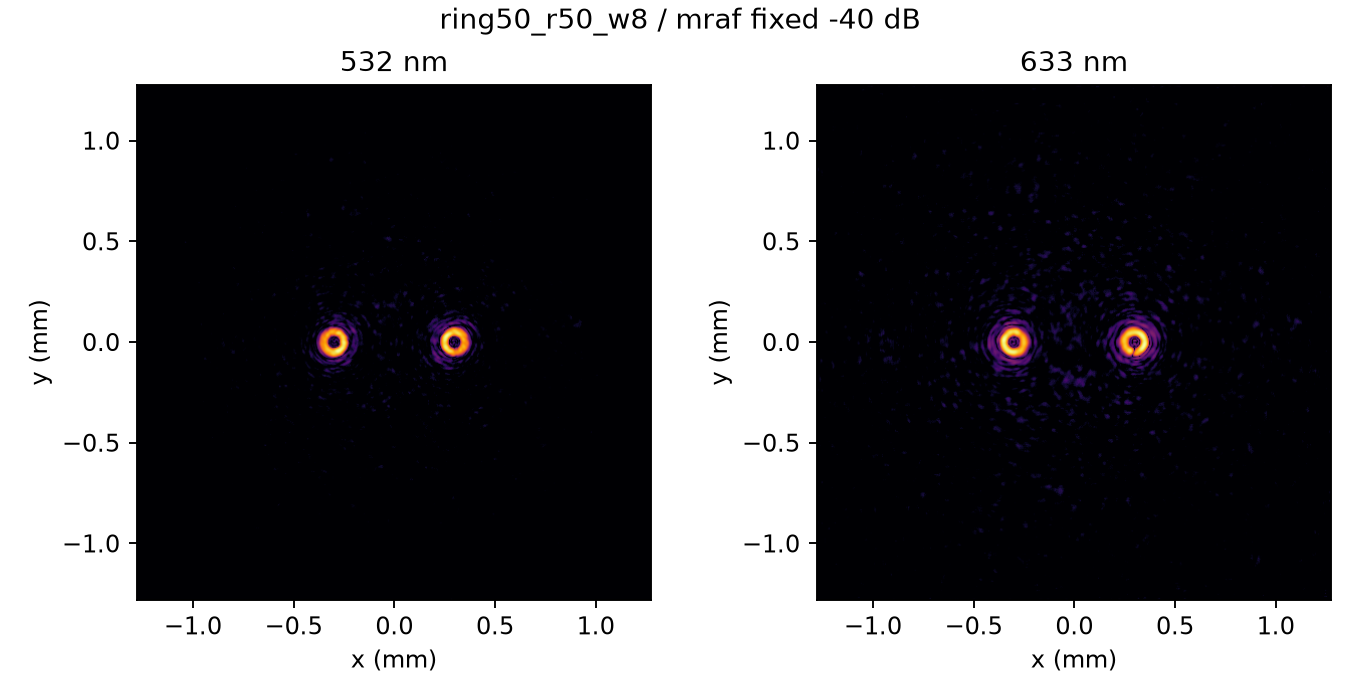
\includegraphics[width=\linewidth]{ring50_output.png}
  \caption{$R=50\,\um$ 输出。}
\end{subfigure}\hfill
\begin{subfigure}{0.31\textwidth}
  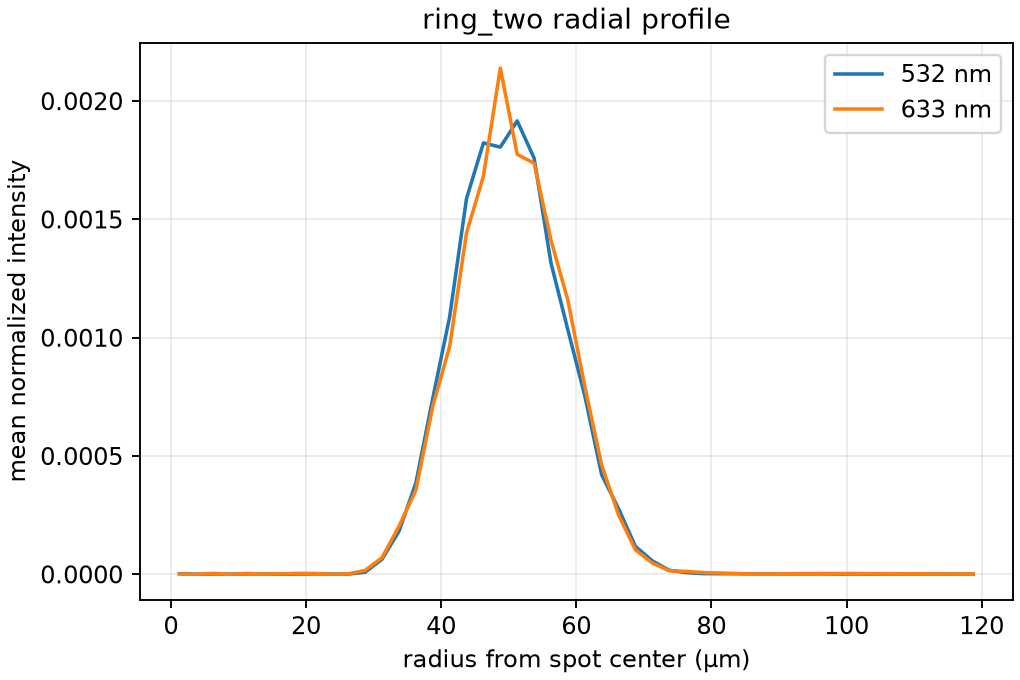
\includegraphics[width=\linewidth]{ring50_profile.png}
  \caption{$R=50\,\um$ 径向剖面。}
\end{subfigure}
\\[0.5em]
\begin{subfigure}{0.31\textwidth}
  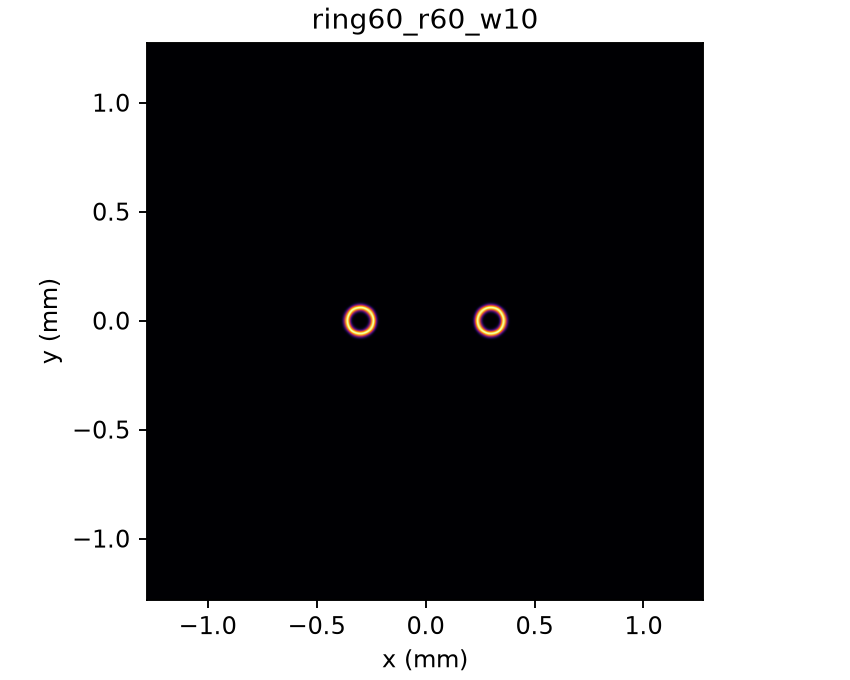
\includegraphics[width=\linewidth]{ring60_target.png}
  \caption{$R=60\,\um$ 目标。}
\end{subfigure}\hfill
\begin{subfigure}{0.31\textwidth}
  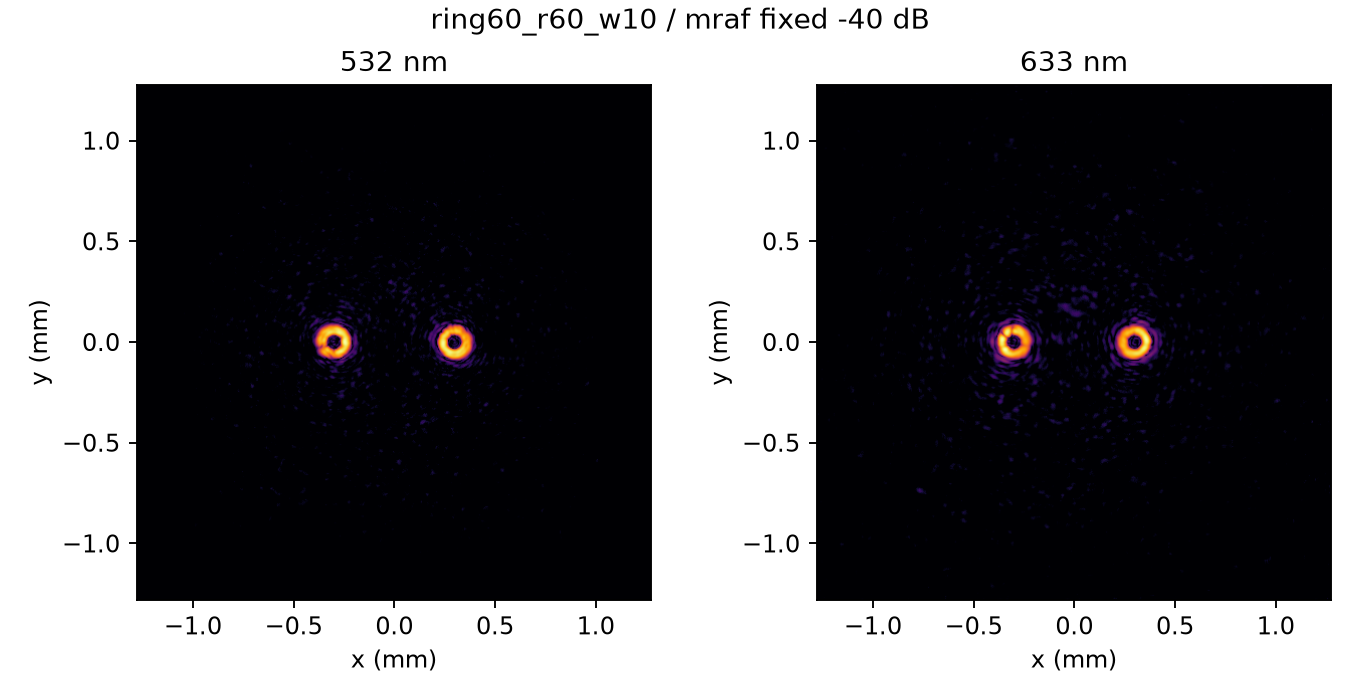
\includegraphics[width=\linewidth]{ring60_output.png}
  \caption{$R=60\,\um$ 输出。}
\end{subfigure}\hfill
\begin{subfigure}{0.31\textwidth}
  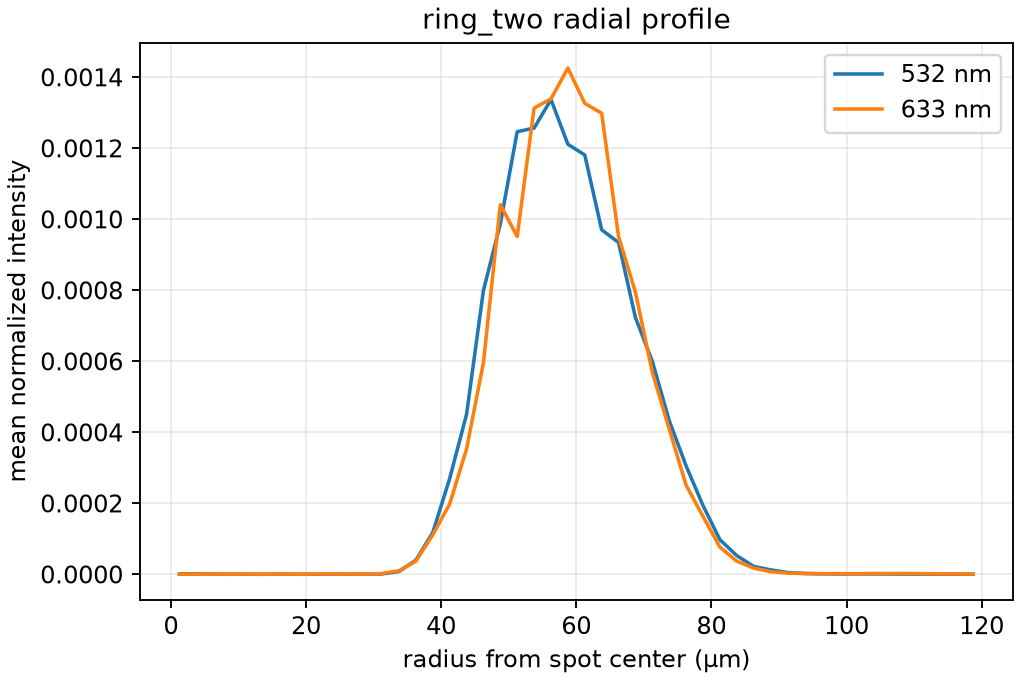
\includegraphics[width=\linewidth]{ring60_profile.png}
  \caption{$R=60\,\um$ 径向剖面。}
\end{subfigure}
\caption{双圆环目标与像面输出。径向曲线用于区分中心空洞、环带峰值和环外背景；仅看固定 dB 图像容易忽略绝对能量和位置漂移。}
\label{fig:ring-results}
\end{figure}

\begin{table}[H]
\centering
\caption{双波长阶段代表性结果的范围。数值来自阶段性正式结果，不包含试跑数据。}
\label{tab:two-wavelength}
\begin{tabular}{lccc}
\toprule
目标 & 最差相关系数 & 背景比例 & 主要跨波长质心漂移 \\
\midrule
双圆斑 & 0.924--0.929 & 0.02--0.03 & 约 \SI{4}{\micro\meter} \\
$R=50\,\um$ 双圆环 & 0.80--0.83 & 约 0.02--0.03 & \SIrange{29}{36}{\micro\meter} \\
$R=60\,\um$ 双圆环 & 0.80--0.83 & 约 0.02--0.03 & \SIrange{34}{36}{\micro\meter} \\
\bottomrule
\end{tabular}
\end{table}

因此，第一阶段的主要结论不是“圆环失败”，而是“圆环形状可以形成，但位置配准比圆斑困难”。这也决定了后续 RGB 消色散实验必须单独记录环半径、内孔泄漏和跨波长质心，而不能只看全场相关系数。

\section{RGB 多图案泛化结果}
\subsection{实验设置}
第二阶段固定波长为 \SI{488}{nm}、\SI{532}{nm} 和 \SI{633}{nm}，在自由传播 \SI{50}{mm} 下比较 Adam 与 MRAF 风格方法。八类目标各使用三个随机种子，粗网格到精网格继承。主比较单元为 $8\times2\times3=48$ 个目标--方法--种子组合；每个单元保留两个候选配置，因此阶段性结果目录实际包含 $96$ 组精细运行，表中报告的是按预定规则选出的代表性配置。

\begin{figure}[H]
\centering
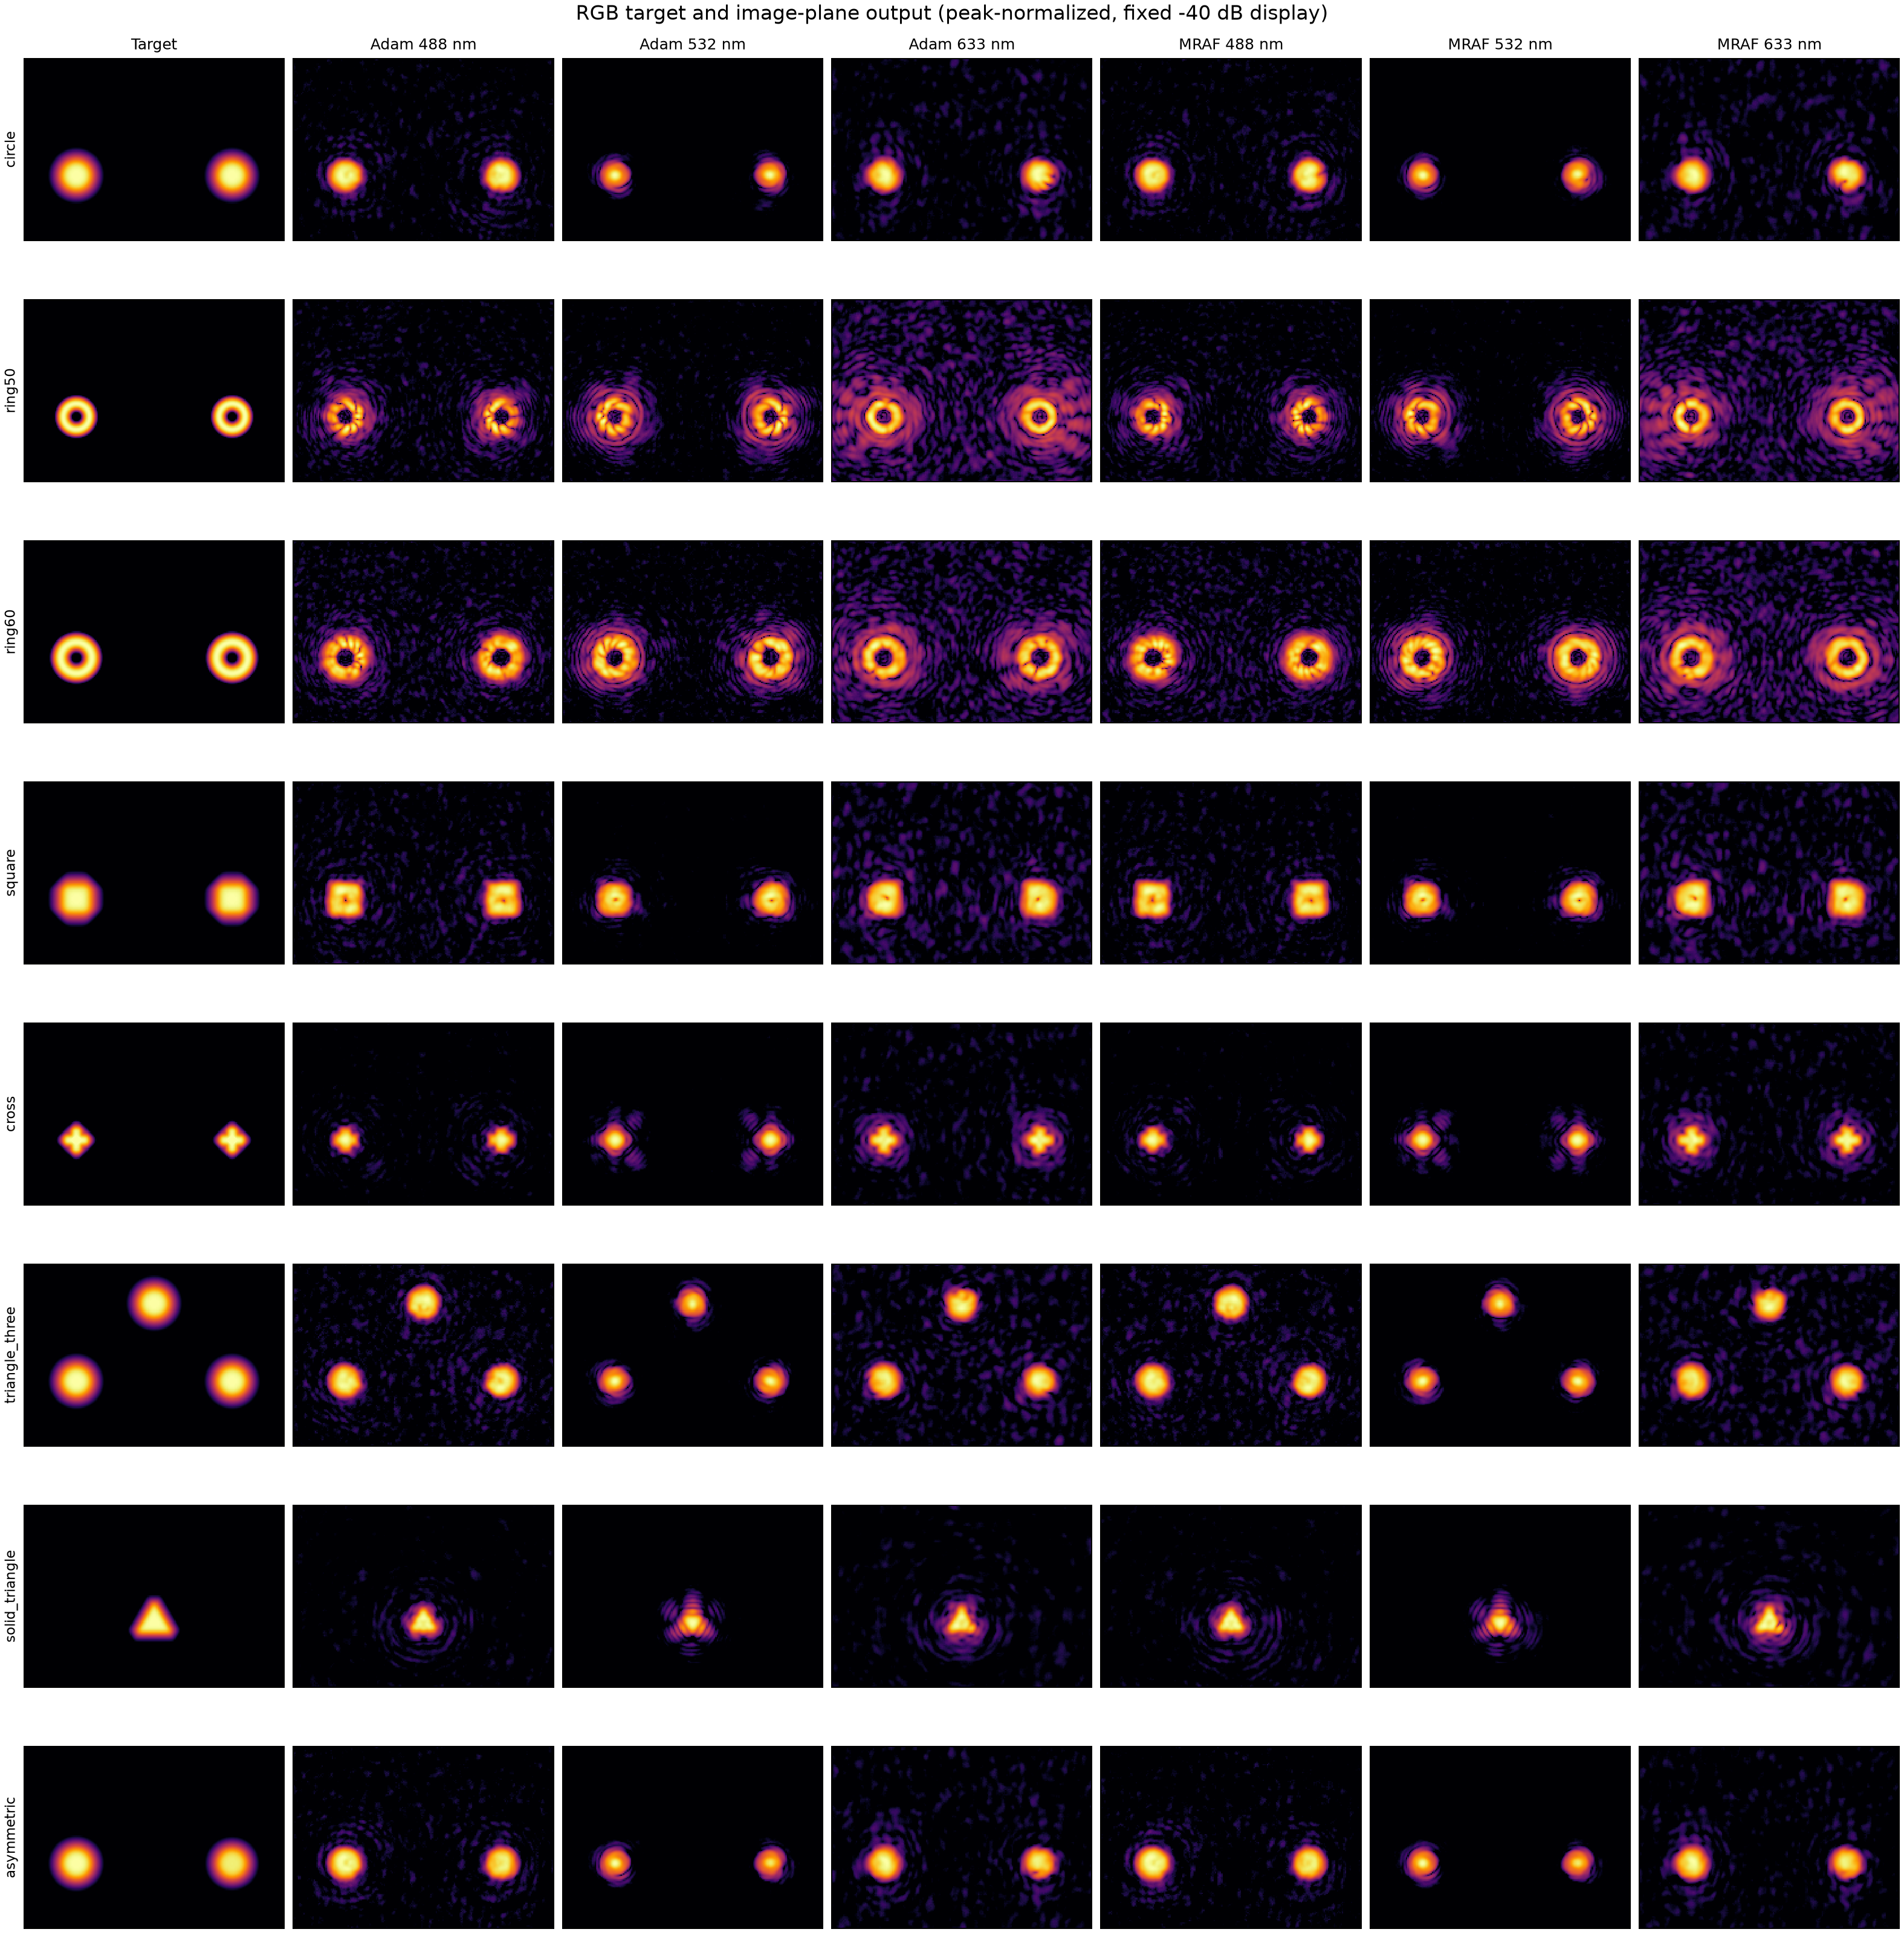
\includegraphics[width=0.98\textwidth]{rgb_generalization_imageplane_comparison.png}
\caption{RGB 多图案泛化的代表性像面比较。每行对应一种目标，输出为固定负四十 dB 显示范围的像面强度。图中可见圆环、十字、方形和三角形均能在一定程度上形成，但边缘和背景质量随波长变化。}
\label{fig:rgb-generalization-images}
\end{figure}

\begin{table}[H]
\centering
\caption{RGB 多图案泛化的正式汇总结果。表中为三种子和波长聚合后的代表性统计；相关系数为最差波长相关系数。}
\label{tab:rgb-generalization}
\resizebox{\textwidth}{!}{%
\begin{tabular}{lccccc}
\toprule
目标 & 方法 & 最差相关系数 & 背景比例 & ROI 效率 & 最大 RGB 质心漂移 / \si{\micro\meter} \\
\midrule
圆斑 & Adam & $0.771\pm0.040$ & 0.038 & 0.937 & 3.2 \\
圆斑 & MRAF 风格 & $0.776\pm0.026$ & 0.036 & 0.940 & 7.7 \\
$R=50\,\um$ 圆环 & Adam & $0.734\pm0.012$ & 0.121 & 0.830 & 24.3 \\
$R=50\,\um$ 圆环 & MRAF 风格 & $0.738\pm0.014$ & 0.122 & 0.830 & 24.4 \\
$R=60\,\um$ 圆环 & Adam & $0.828\pm0.033$ & 0.083 & 0.863 & 8.1 \\
$R=60\,\um$ 圆环 & MRAF 风格 & $0.832\pm0.032$ & 0.088 & 0.857 & 5.1 \\
方形 & Adam & $0.811\pm0.024$ & 0.035 & 0.939 & 5.3 \\
方形 & MRAF 风格 & $0.810\pm0.022$ & 0.034 & 0.940 & 5.1 \\
十字 & Adam & $0.890\pm0.004$ & 0.055 & 0.895 & 2.0 \\
十字 & MRAF 风格 & $0.889\pm0.002$ & 0.053 & 0.898 & 2.8 \\
三角形三圆斑 & Adam & $0.786\pm0.012$ & 0.036 & 0.943 & 9.3 \\
三角形三圆斑 & MRAF 风格 & $0.788\pm0.018$ & 0.037 & 0.942 & 6.8 \\
实心三角形 & Adam & $0.798\pm0.005$ & 0.059 & 0.871 & 2.1 \\
实心三角形 & MRAF 风格 & $0.797\pm0.007$ & 0.060 & 0.869 & 2.3 \\
不对称双斑 & Adam & $0.776\pm0.055$ & 0.040 & 0.933 & 5.3 \\
不对称双斑 & MRAF 风格 & $0.780\pm0.053$ & 0.039 & 0.935 & 5.2 \\
\bottomrule
\end{tabular}}
\end{table}

十字是本轮表现较好的非圆形目标，最差相关系数接近 $0.89$，背景约为 $0.05$，且 RGB 质心漂移约为 \SIrange{2}{3}{\micro\meter}。$R=60\,\um$ 圆环明显优于 $R=50\,\um$ 圆环，说明增大环半径和环带可分辨尺度有助于降低采样和传播模糊。相比之下，$R=50\,\um$ 圆环的背景和质心漂移同时偏大，说明其难点不仅是“环中心是否为空”，还包括多波长下环带的横向配准。

\begin{figure}[H]
\centering
\begin{subfigure}{0.48\textwidth}
  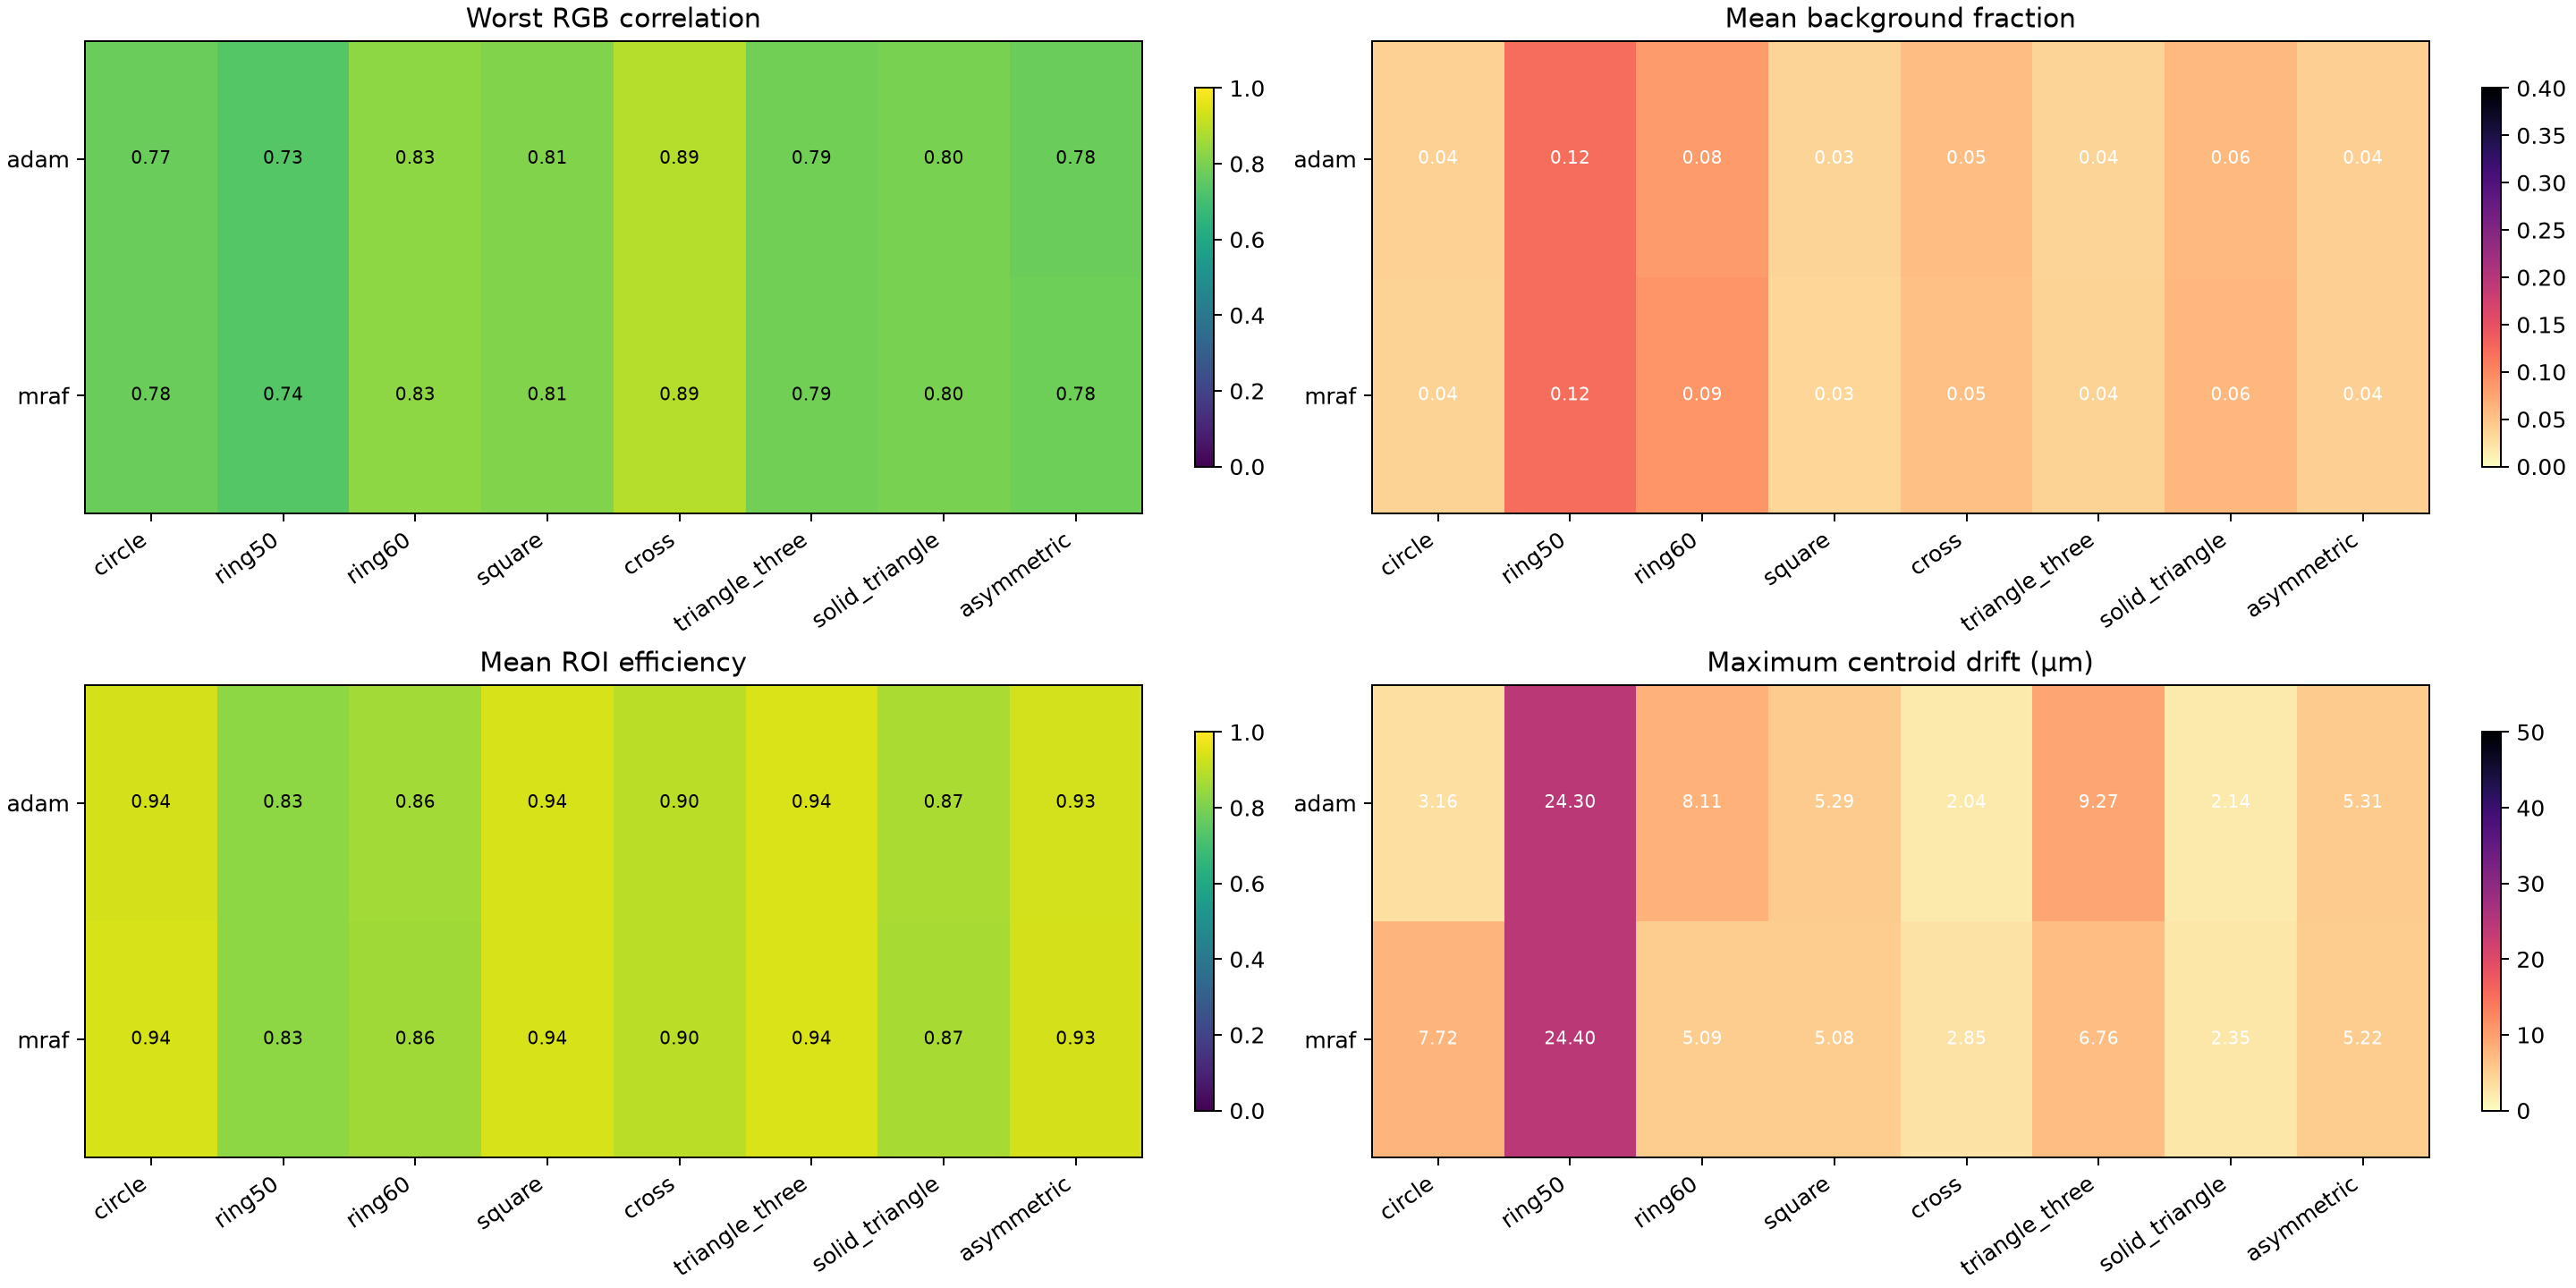
\includegraphics[width=\linewidth]{rgb_generalization_metric_heatmaps.png}
  \caption{指标热图。}
\end{subfigure}\hfill
\begin{subfigure}{0.48\textwidth}
  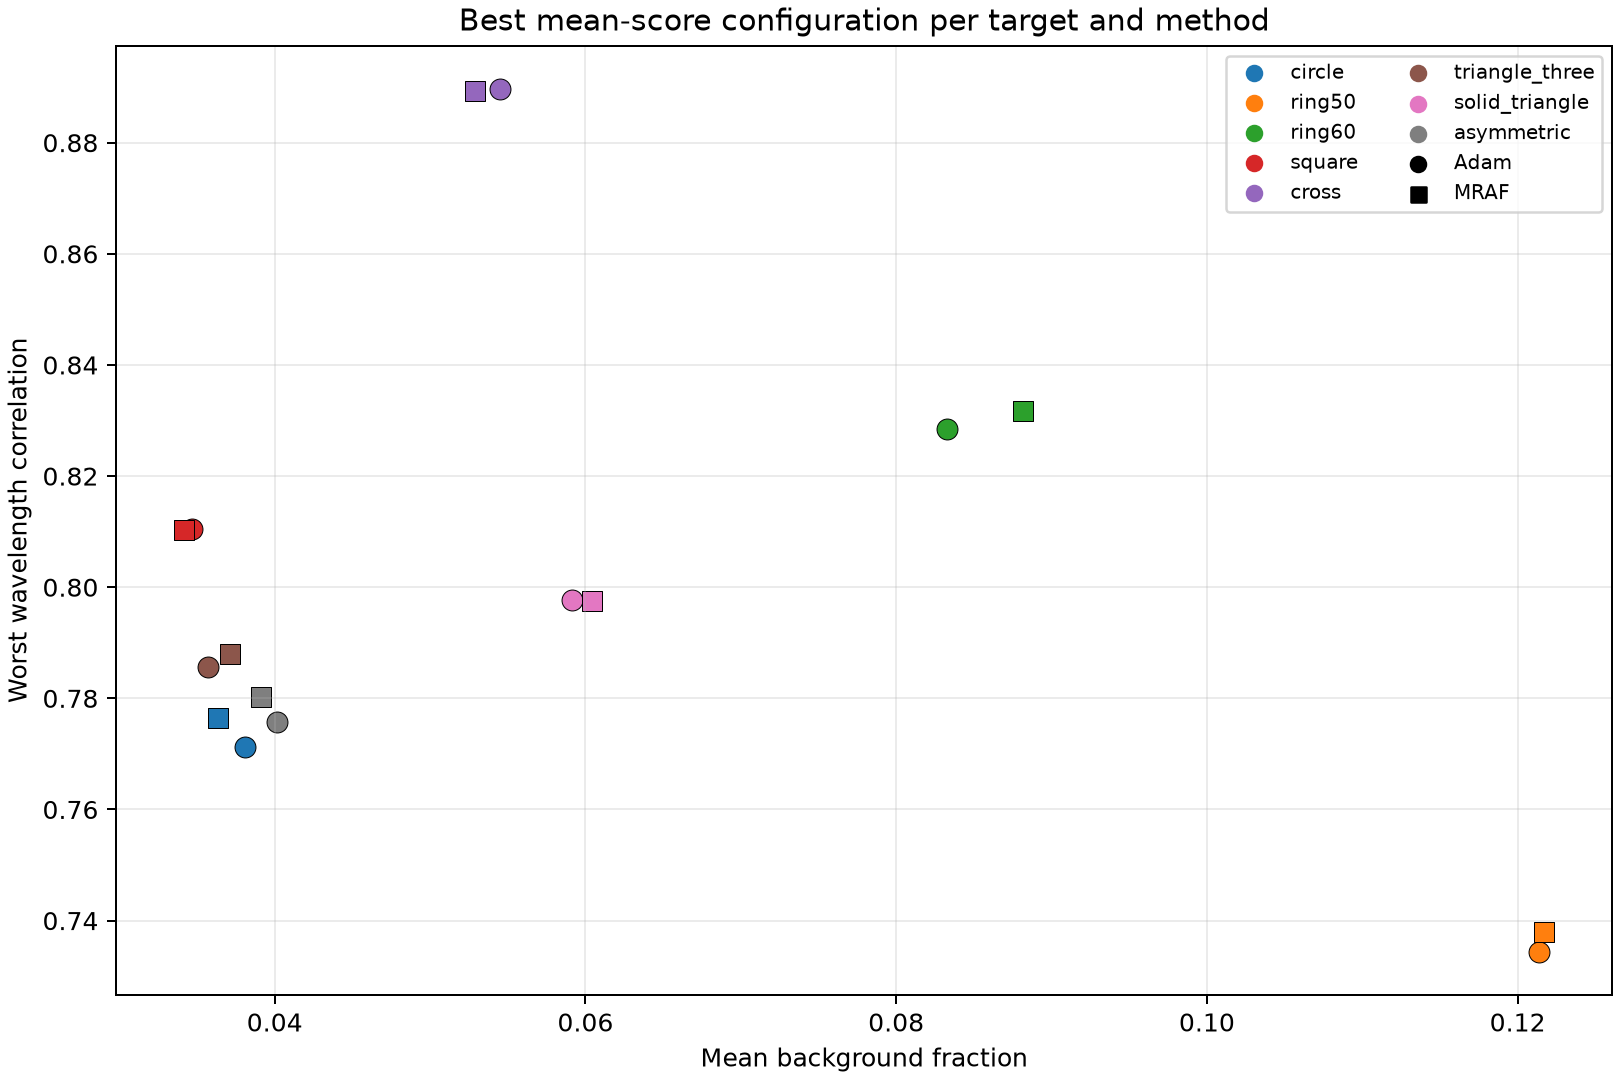
\includegraphics[width=\linewidth]{rgb_generalization_pareto.png}
  \caption{相关系数--背景 Pareto 图。}
\end{subfigure}
\caption{RGB 多目标泛化的综合比较。不同目标的难度不能由一个统一的相关系数阈值完全概括。}
\label{fig:rgb-generalization-metrics}
\end{figure}

总体上，第二阶段支持“有限图案集合上的方法可迁移”，但不支持“对任意图案具有泛化能力”。方形、三角形和十字能够形成可识别结构，但边界距离、顶点误差、尖角钝化和边缘粗糙度尚未全部纳入统一的几何损失，因此不能只根据全场相关系数宣称几何重建已经完成。MRAF 风格方法相对 Adam 的最佳配置平均分差约为 $0.001$，差异小且随目标变化，不能据此判定 MRAF 普遍优于 Adam。

\subsection{共同色标与绝对能量评价}
前期实验中，如果每个波长都按自身峰值显示，RGB 图像可能看起来比实际更接近。为此，单独完成了共同线性色标、共同 dB 色标和形状归一化三套图像，并保留输入能量、像面裁剪能量、ROI 绝对能量和背景绝对能量。等入射功率 $P_{488}:P_{532}:P_{633}=1:1:1$ 只作为当前数值实验的默认假设，不是 CIE 色度学或真实激光功率模型。

\begin{figure}[H]
\centering
\begin{subfigure}{0.49\textwidth}
  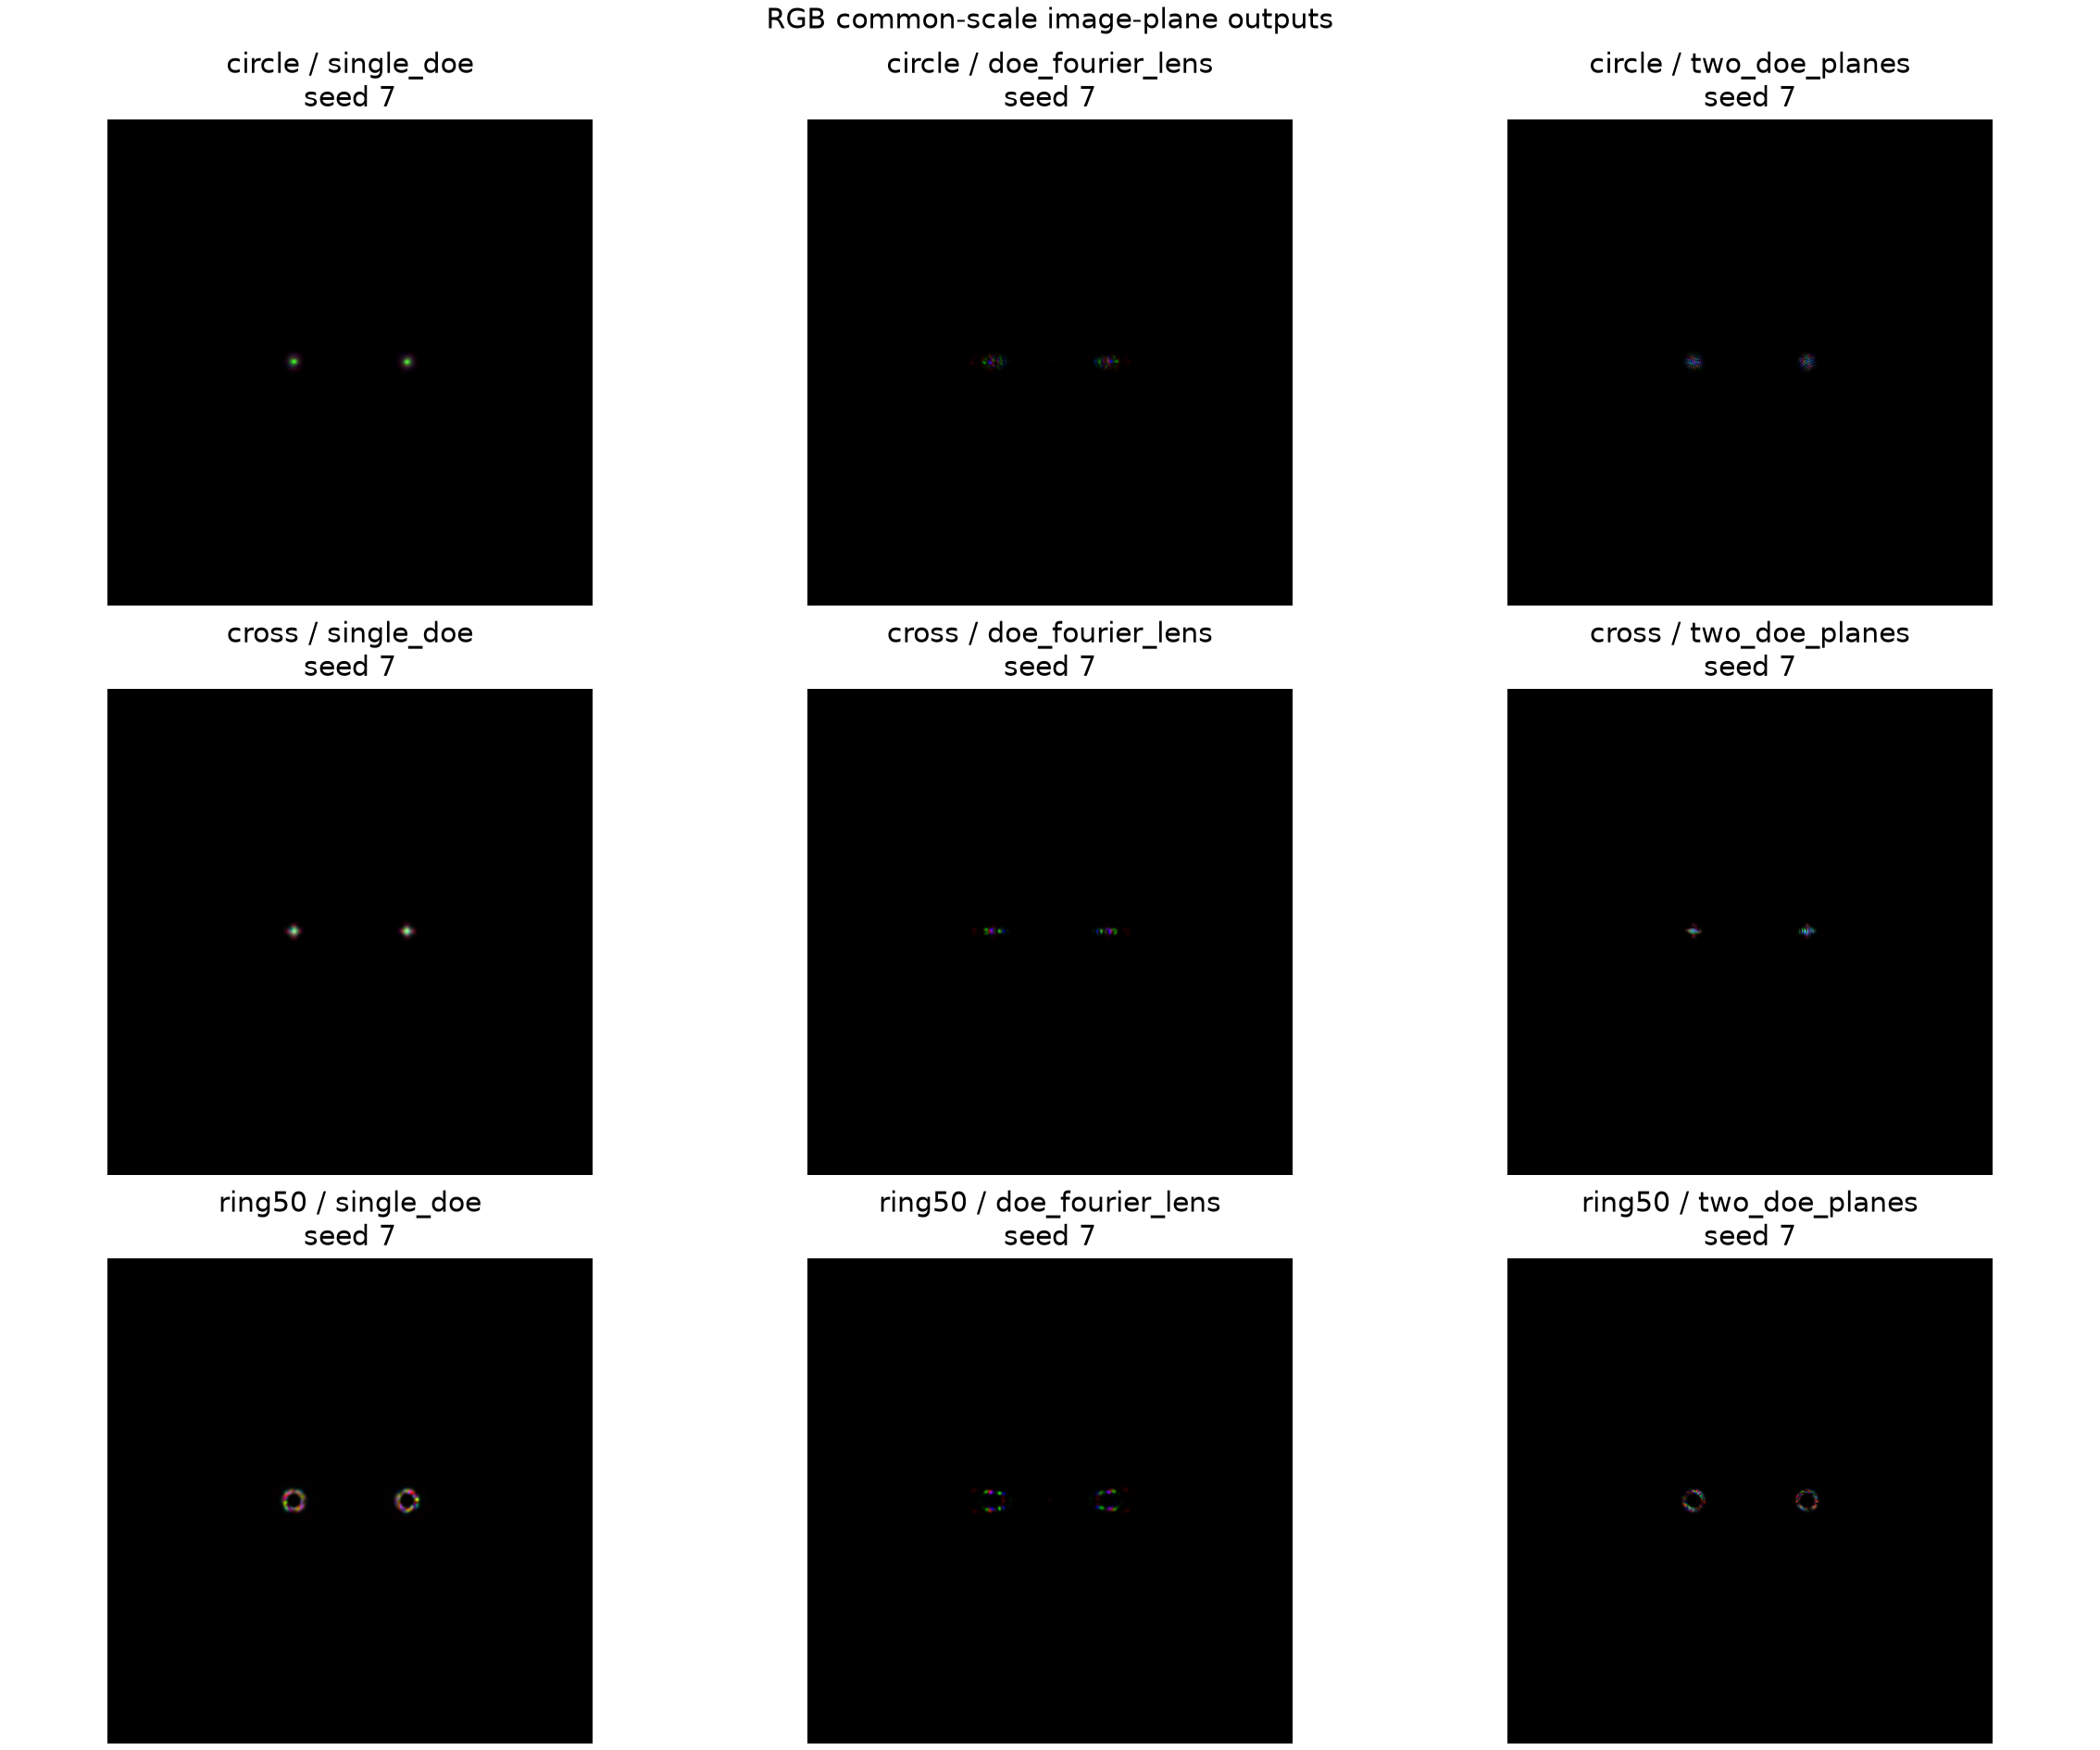
\includegraphics[width=\linewidth]{rgb_eval_common_scale.png}
  \caption{共同线性色标。}
\end{subfigure}\hfill
\begin{subfigure}{0.49\textwidth}
  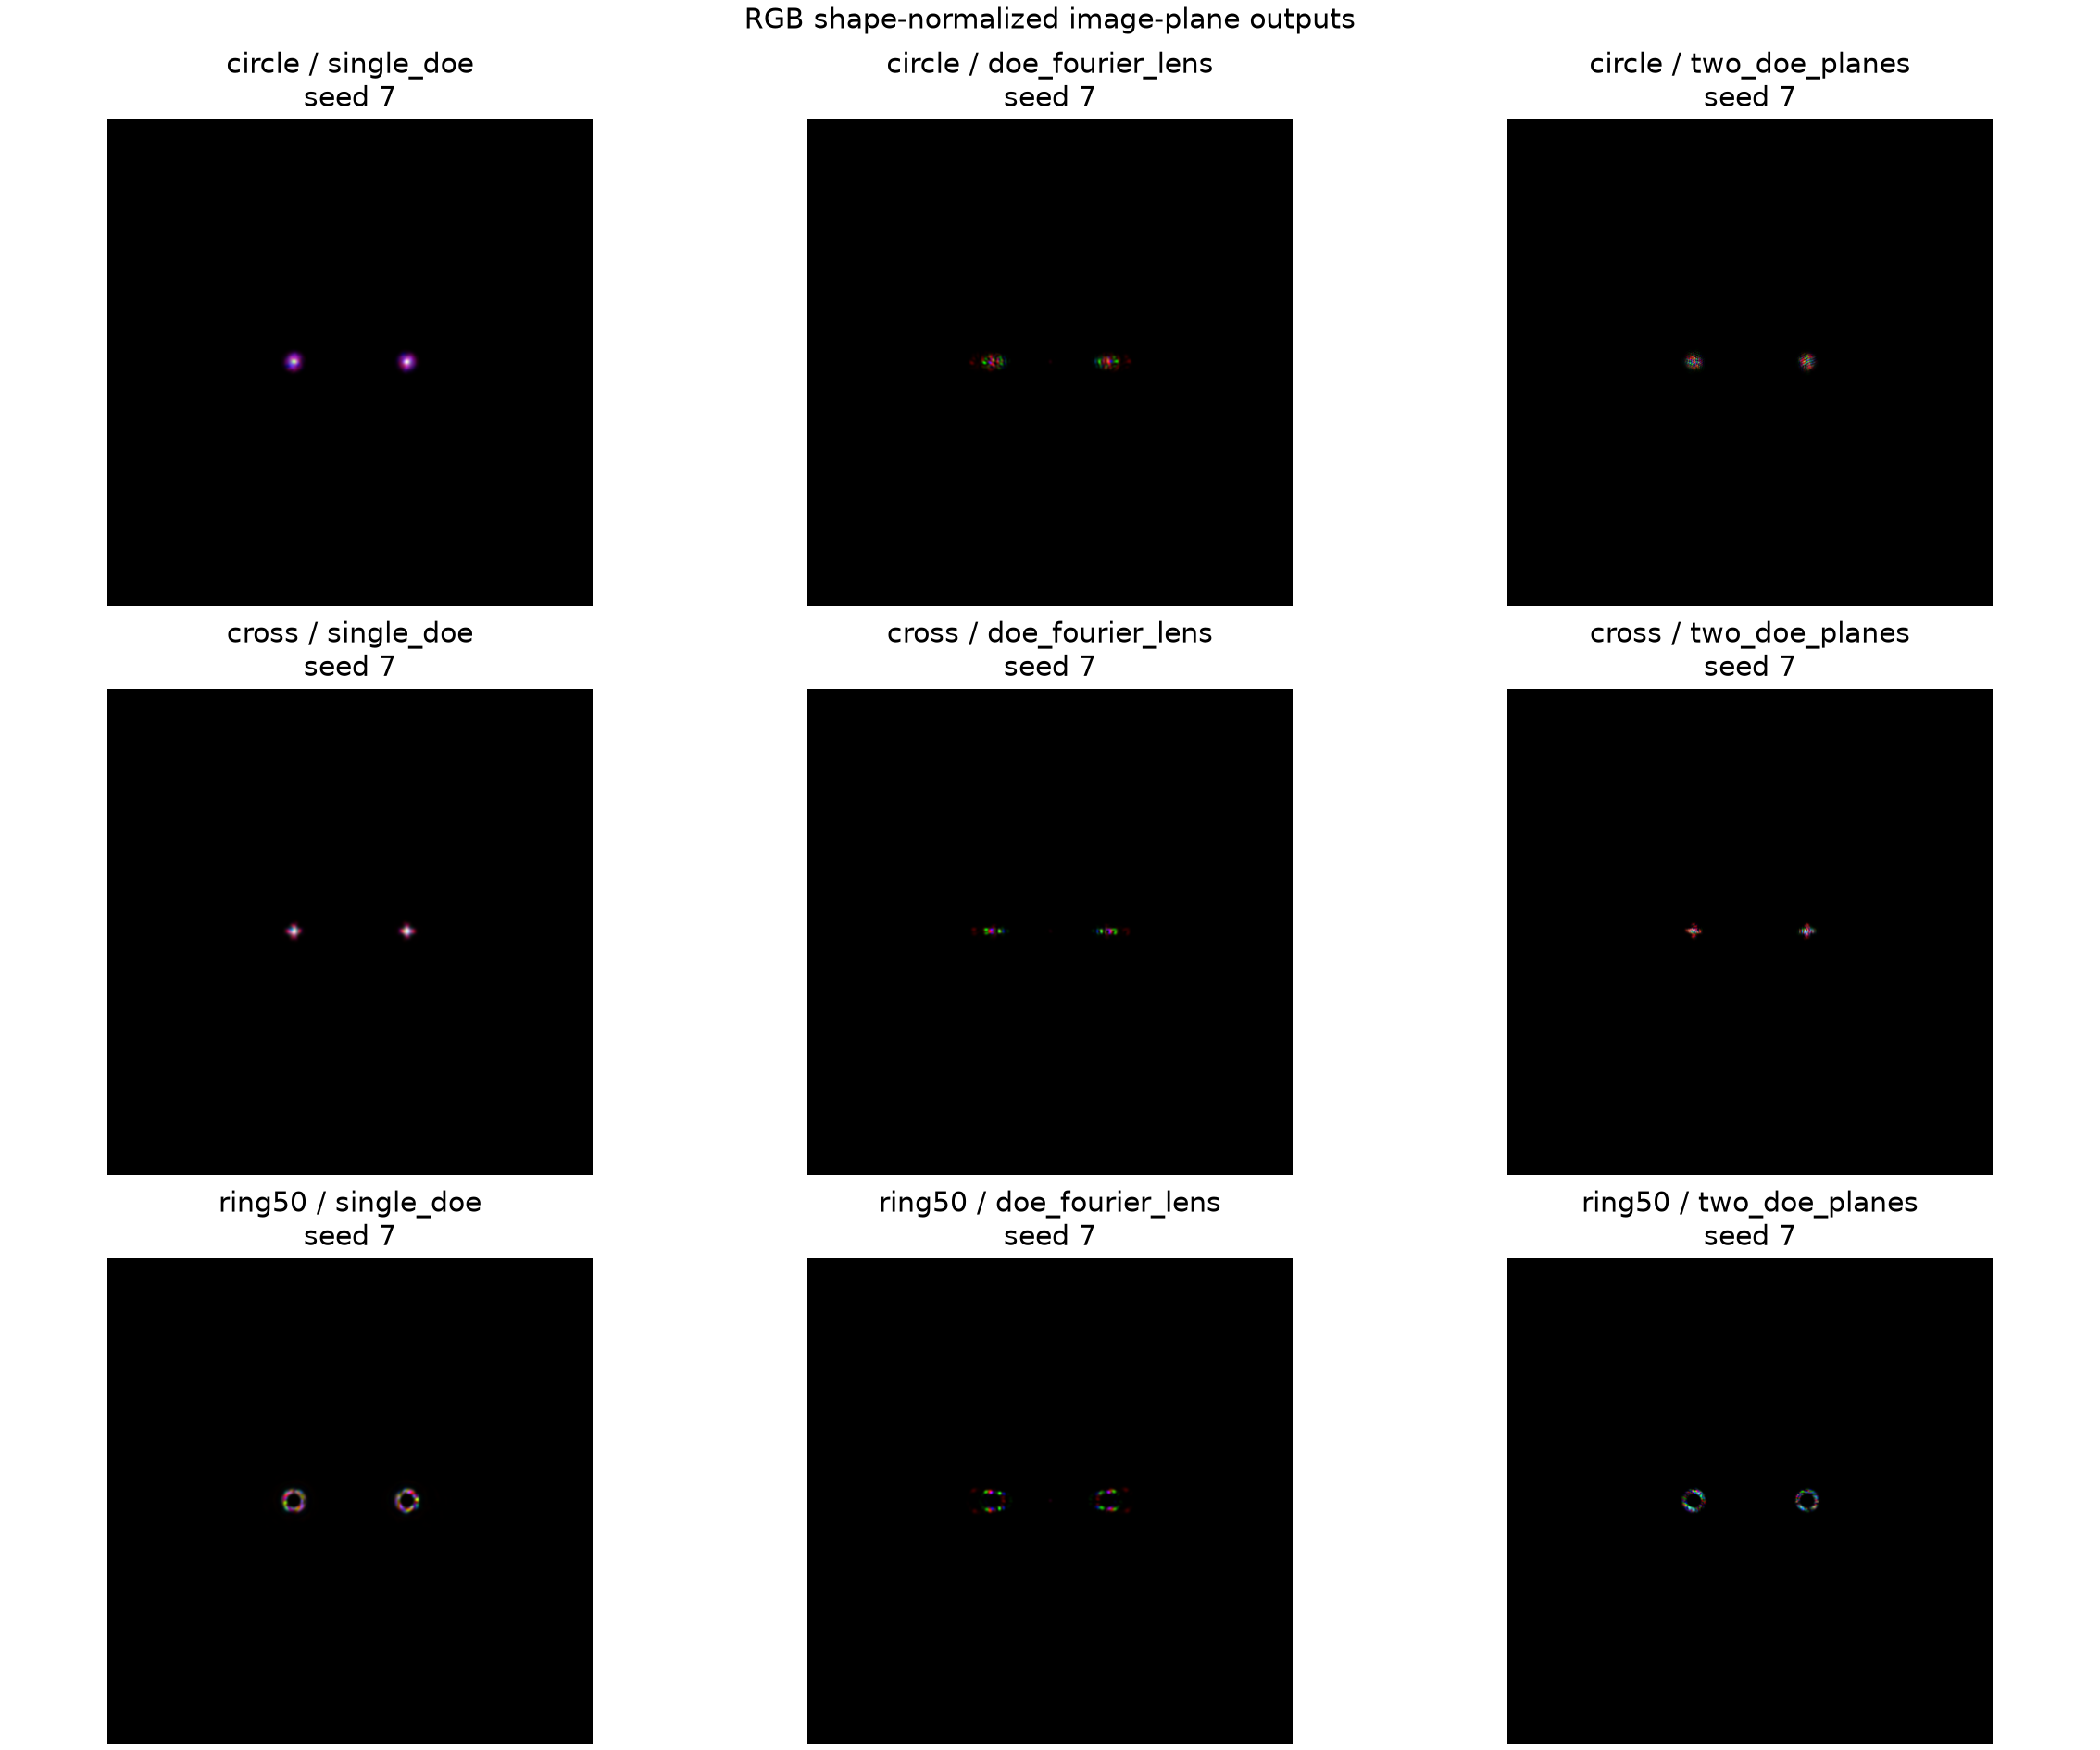
\includegraphics[width=\linewidth]{rgb_eval_shape_normalized.png}
  \caption{单通道形状归一化。}
\end{subfigure}
\caption{共同色标与形状归一化的区别。前者保留通道能量差，后者只用于观察空间形状。}
\label{fig:common-scale}
\end{figure}

\section{RGB 跨波长消色散损失消融}
\subsection{消融设计}
在第三阶段，移除 \texttt{doe\_fourier\_lens} 主线，只保留单 DOE 与双 DOE 两种架构。固定目标为圆斑、十字和 $R=50\,\um$ 圆环，波长为 488/532/633 nm，输入功率为 1:1:1。新增损失包含五类跨波长约束：
\begin{enumerate}
\item 共同尺度 ROI 内的逐像素形状一致性和绝对强度一致性；
\item 过渡区振幅梯度一致性；
\item 背景区的 RGB 强度一致性；
\item RGB ROI 绝对效率的变异系数惩罚；
\item 多组件能量比例在波长之间的一致性。
\end{enumerate}
新增权重在前 $25\%$ 迭代中关闭，在 $25\%$--$75\%$ 之间线性增加，后 $25\%$ 使用完整权重。七个消融变体为 baseline、pixel、edge、background、energy、component 和 full；每个变体包含 $3$ 个目标、$2$ 种光路和 $3$ 个随机种子，共 $126$ 次完整运行。粗阶段使用 $256\times256$、120 次迭代，精阶段使用 $512\times512$、400 次迭代。GPU 为 NVIDIA GeForce RTX 5060 Ti，总记录运行时间约为 $1805$ 秒；所有运行均未发现 NaN 或 Inf。

\begin{table}[H]
\centering
\caption{RGB 消色散消融变体及对应问题。}
\label{tab:ablation-groups}
\begin{tabular}{ll}
\toprule
变体 & 主要研究问题 \\
\midrule
baseline & 没有跨波长一致性损失时的基线 \\
pixel & 是否改善共同尺度 ROI 的像素纹理和绝对强度 \\
edge & 是否减少 RGB 边缘毛刺和色边 \\
background & 是否降低单通道背景噪声 \\
energy & 是否降低 RGB ROI 绝对功率差 \\
component & 是否稳定左右组件的颜色比例 \\
full & 多项一致性损失联合时的综合效果 \\
\bottomrule
\end{tabular}
\end{table}

\subsection{主要结果}
图\ref{fig:decolorization-overview}给出了 full 变体的共同色标/形状归一化像面概览。和单独按峰值归一化的旧图相比，共同色标能直接看到三色能量和背景的真实差异。

\begin{figure}[H]
\centering
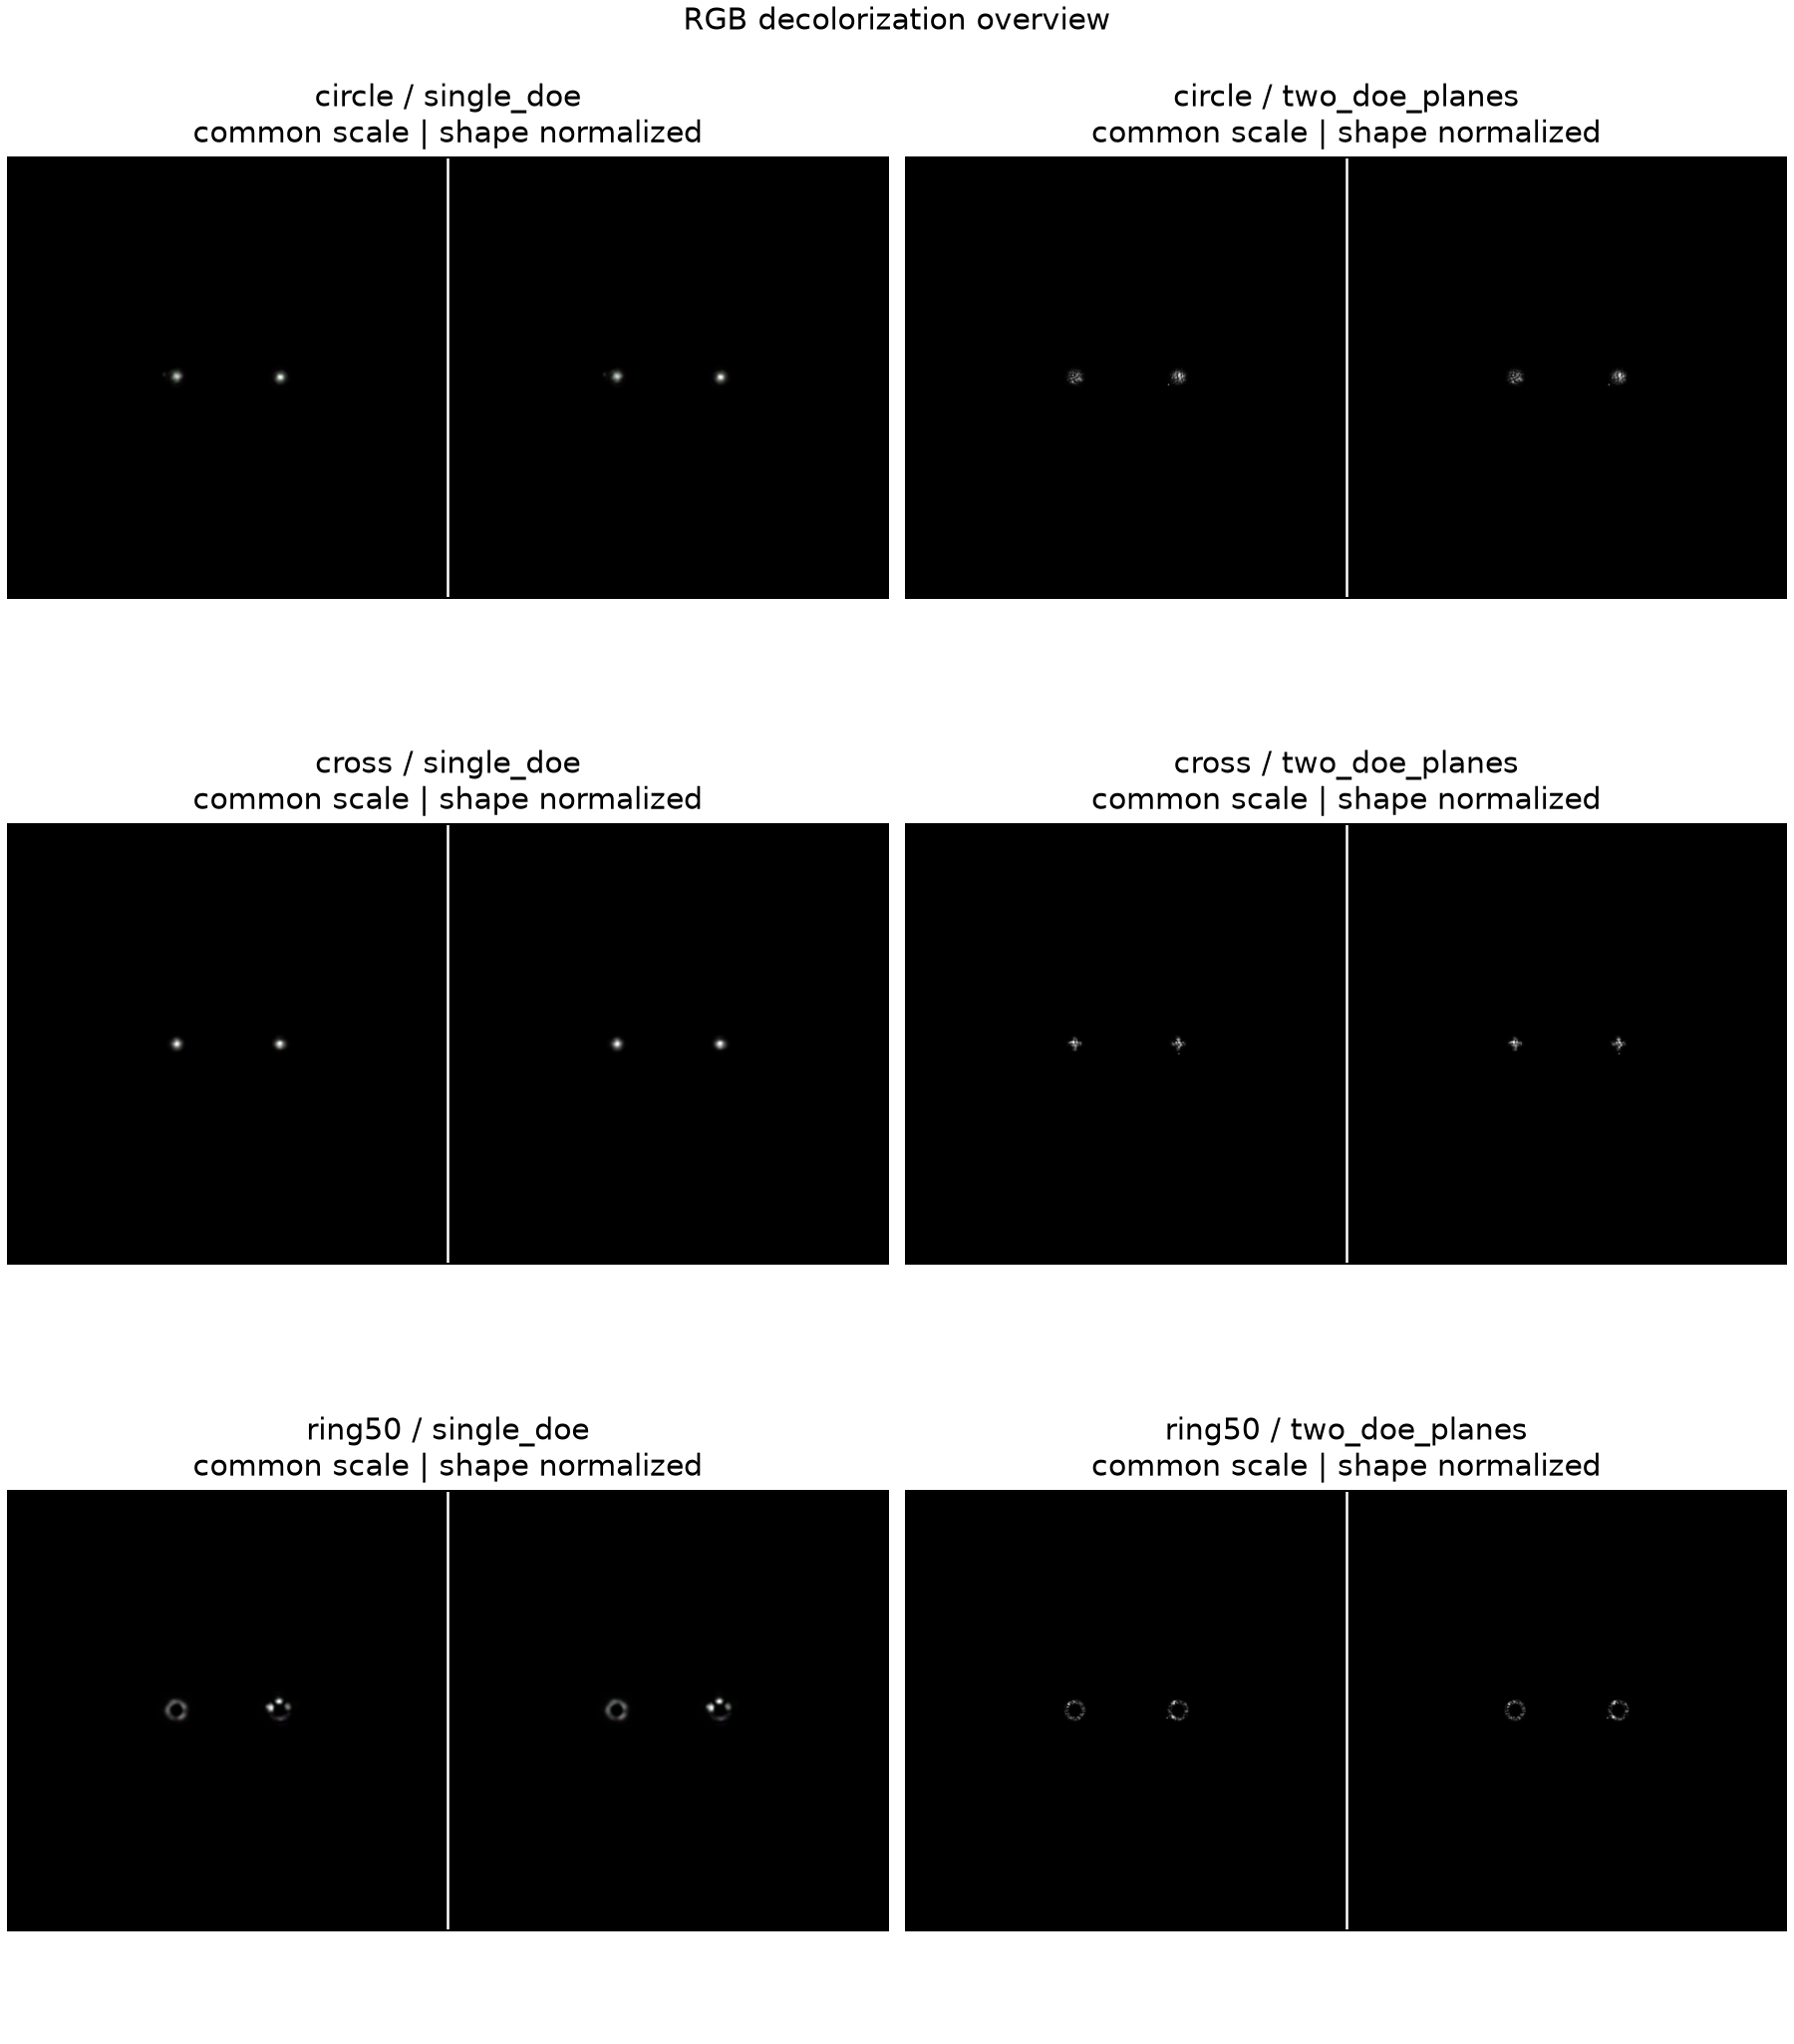
\includegraphics[width=0.97\textwidth]{decolorization_overview.png}
\caption{RGB 消色散正式实验的像面概览。每个目标--光路单元的图像包含共同尺度与形状归一化信息；本图使用正式 $512\times512$ 精网格结果。}
\label{fig:decolorization-overview}
\end{figure}

\begin{table}[H]
\centering
\caption{baseline 与 full 的六个目标--光路单元对照。Pearson 为共同尺度 ROI Pearson，CV 为 RGB ROI 能量变异系数，$C_{\mathrm{worst}}$ 为最差波长相关系数。}
\label{tab:decolorization-main}
\resizebox{\textwidth}{!}{%
\begin{tabular}{lccrrrrrr}
\toprule
目标 & 光路 & Pearson$_{\mathrm{base}}$ & Pearson$_{\mathrm{full}}$ & CV$_{\mathrm{base}}$ & CV$_{\mathrm{full}}$ & $C_{\mathrm{worst,base}}$ & $C_{\mathrm{worst,full}}$ & 背景 full \\
\midrule
圆斑 & 单 DOE & 0.780 & 0.998 & 0.097 & 0.020 & 0.763 & 0.866 & 0.102 \\
圆斑 & 双 DOE & 0.418 & 0.996 & 0.147 & 0.003 & 0.751 & 0.855 & 0.180 \\
十字 & 单 DOE & 0.832 & 0.999 & 0.086 & 0.011 & 0.869 & 0.907 & 0.110 \\
十字 & 双 DOE & 0.566 & 0.997 & 0.159 & 0.003 & 0.803 & 0.883 & 0.196 \\
$R=50\,\um$ 圆环 & 单 DOE & 0.237 & 0.994 & 0.196 & 0.008 & 0.798 & 0.796 & 0.193 \\
$R=50\,\um$ 圆环 & 双 DOE & 0.327 & 0.996 & 0.086 & 0.003 & 0.775 & 0.831 & 0.215 \\
\bottomrule
\end{tabular}}
\end{table}

表\ref{tab:decolorization-main}给出了本研究最重要的定量证据。首先，full 变体在六个单元中共同尺度 ROI Pearson 均提高超过 $0.10$，增量约为 $0.17$--$0.76$。其次，RGB ROI 能量 CV 在六个单元中均下降超过 $20\%$，实际降幅约为 $79\%$--$98\%$。第三，最差波长图案相关系数没有出现超过 $0.05$ 的下降；十字和圆斑反而有所提高，$R=50\,\um$ 单 DOE 圆环基本不变，双 DOE 圆环得到改善。第四，最大组件质心漂移均下降到约 \SIrange{0.2}{1.2}{\micro\meter} 量级。

但是，full 不是无代价的成功。baseline 到 full 的平均背景比例变化分别约为：圆斑单 DOE $+0.042$、圆斑双 DOE $+0.076$、十字单 DOE $+0.023$、十字双 DOE $+0.072$、$R=50\,\um$ 圆环单 DOE $+0.032$、圆环双 DOE $+0.067$。按预设的“背景增加不超过 $0.03$”标准，只有十字单 DOE 单元满足，六个单元整体不满足。这说明像素一致性和能量平衡损失确实把三色拉到了相似的空间结构和绝对能量水平，但部分自由度是以更高背景为代价换来的。

\begin{figure}[H]
\centering
\begin{subfigure}{0.48\textwidth}
  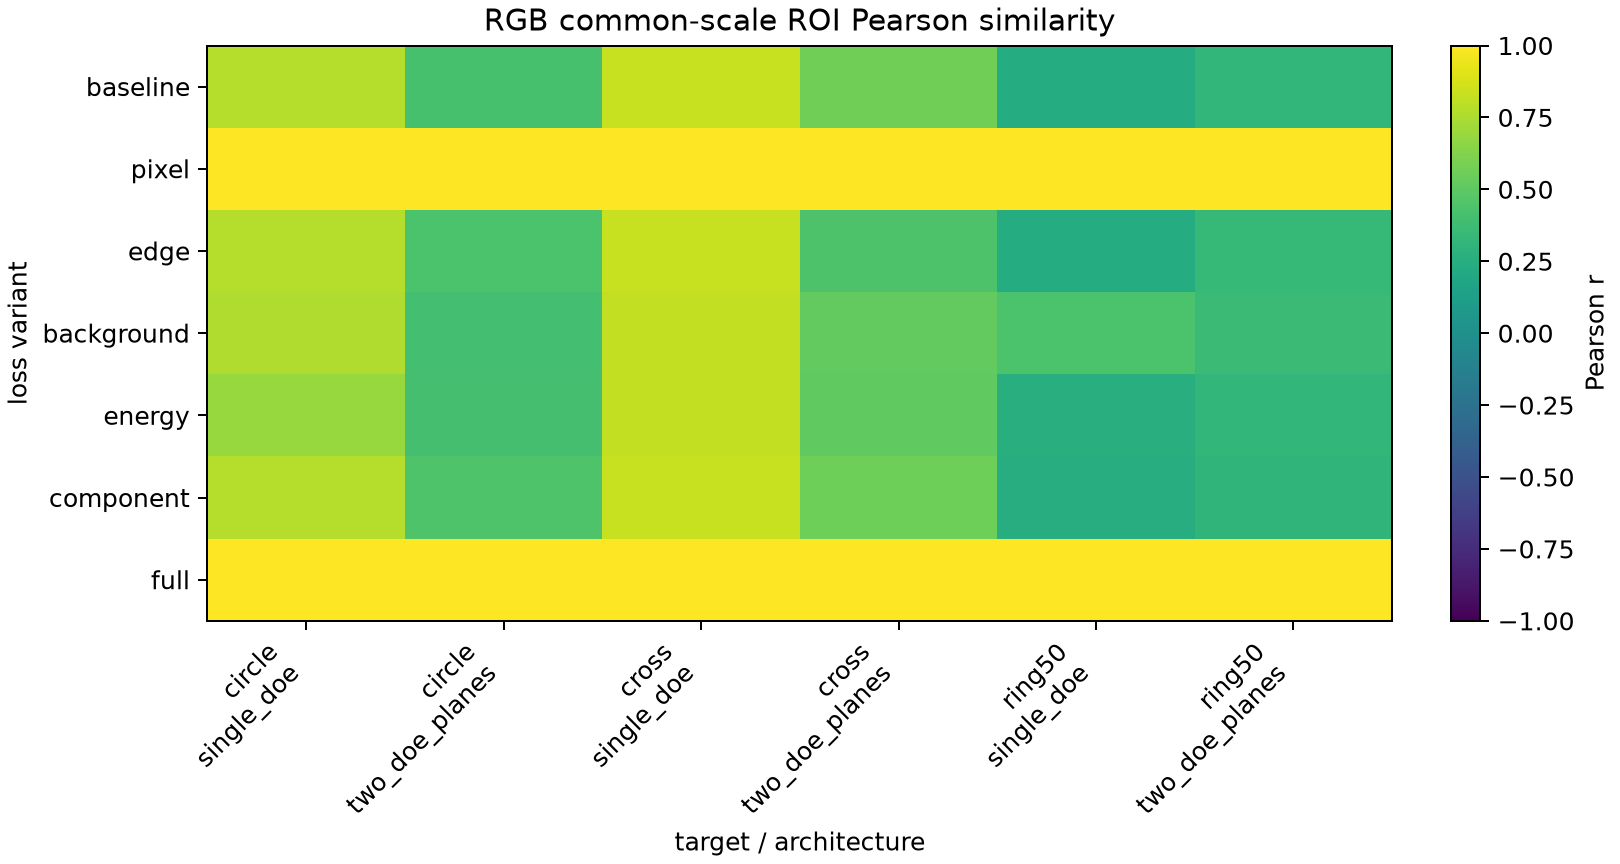
\includegraphics[width=\linewidth]{decolorization_pixel_heatmap.png}
  \caption{共同尺度像素相似度。}
\end{subfigure}\hfill
\begin{subfigure}{0.48\textwidth}
  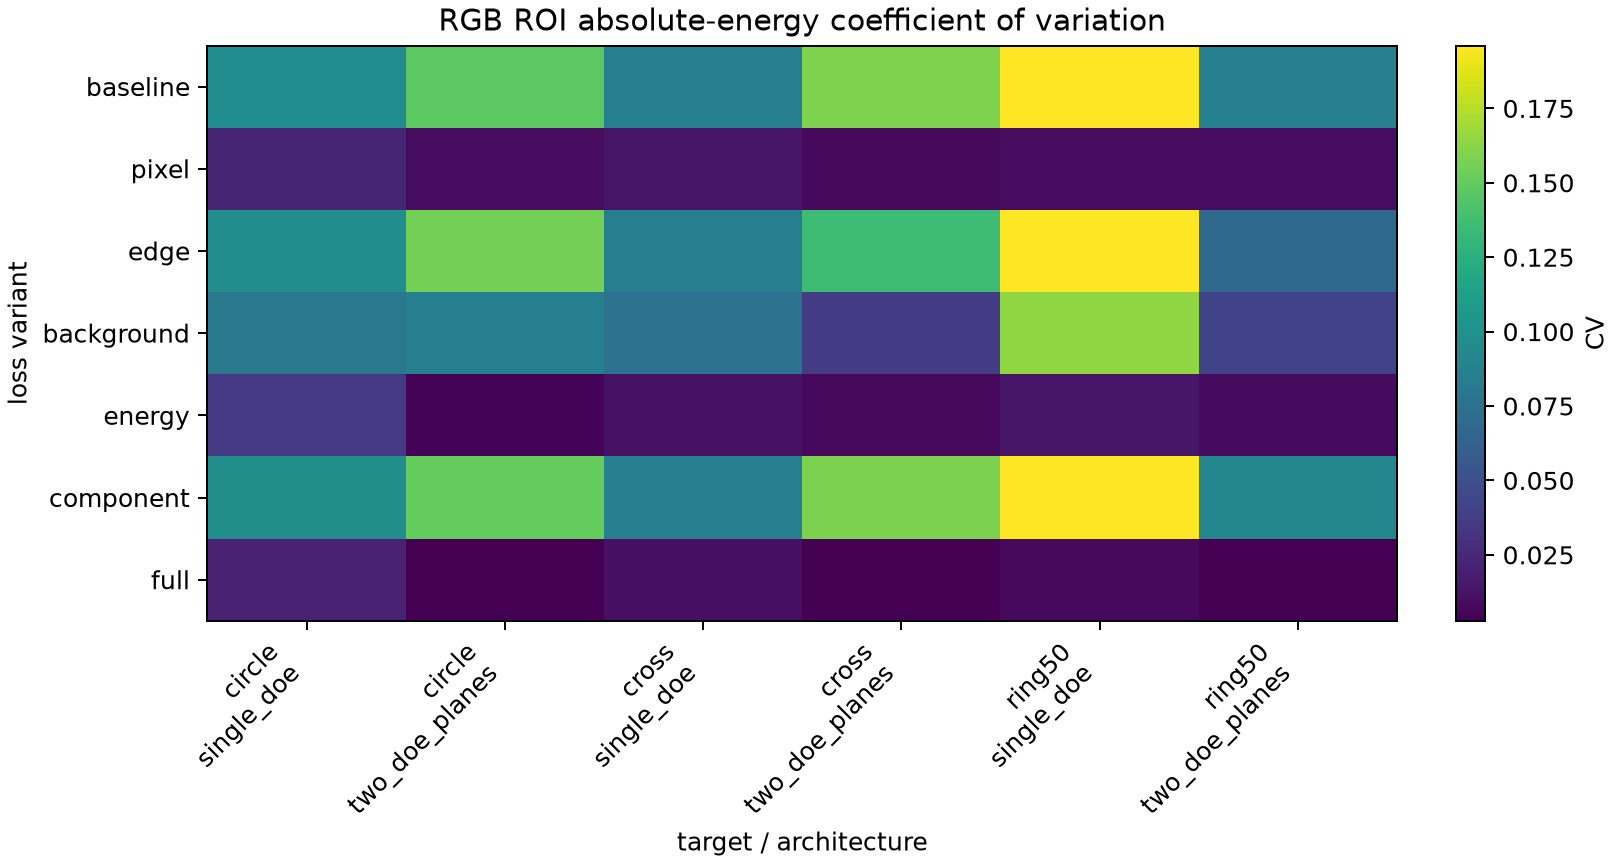
\includegraphics[width=\linewidth]{decolorization_energy_cv_heatmap.png}
  \caption{RGB 能量 CV。}
\end{subfigure}
\\[0.5em]
\begin{subfigure}{0.48\textwidth}
  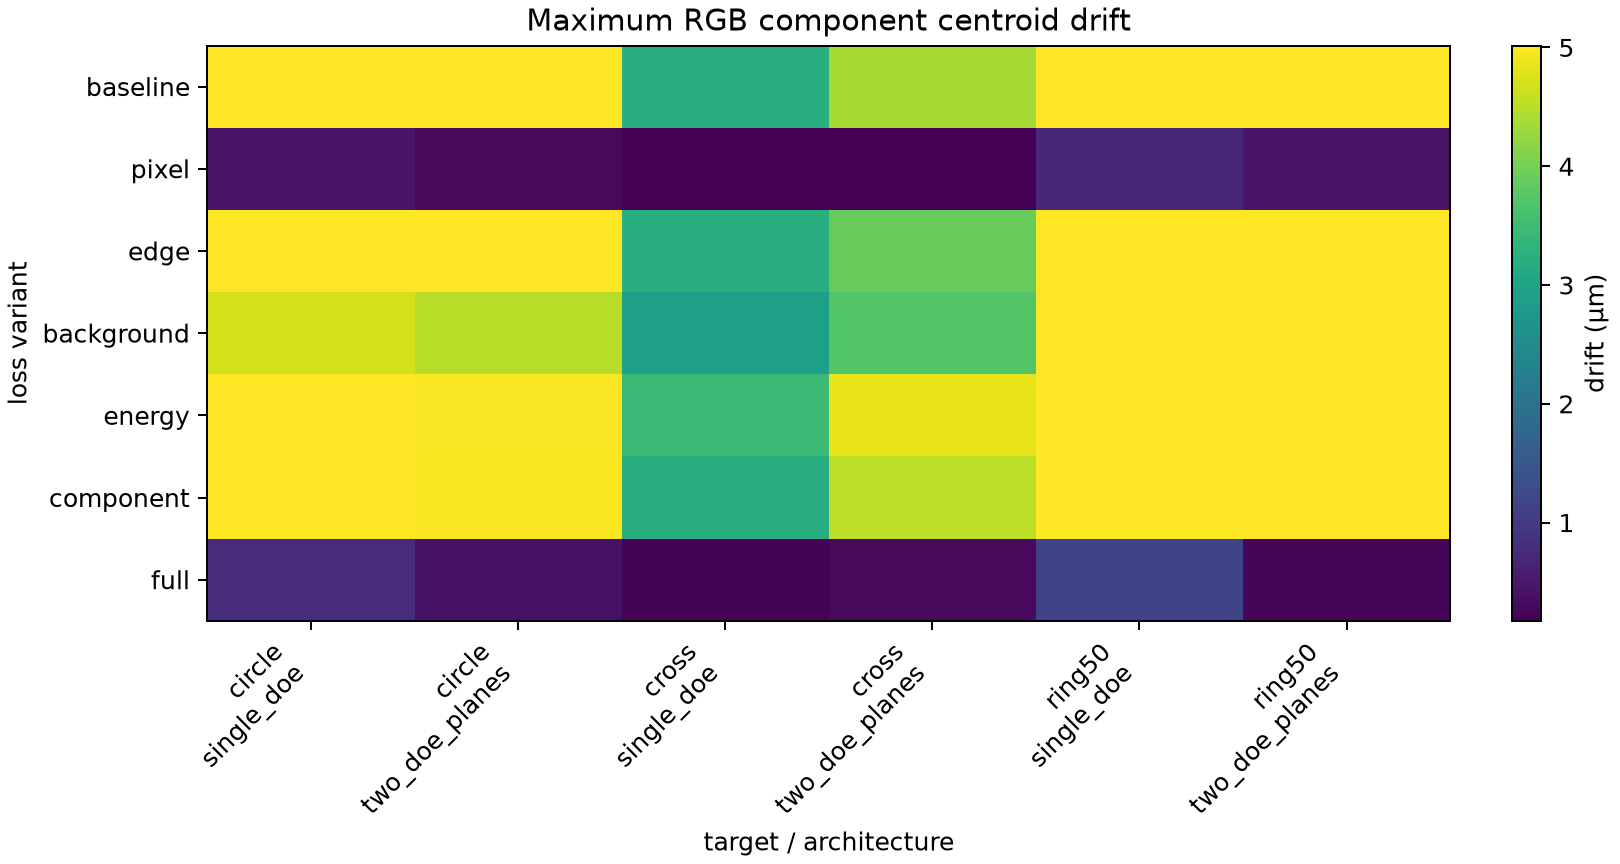
\includegraphics[width=\linewidth]{decolorization_centroid_heatmap.png}
  \caption{质心漂移。}
\end{subfigure}\hfill
\begin{subfigure}{0.48\textwidth}
  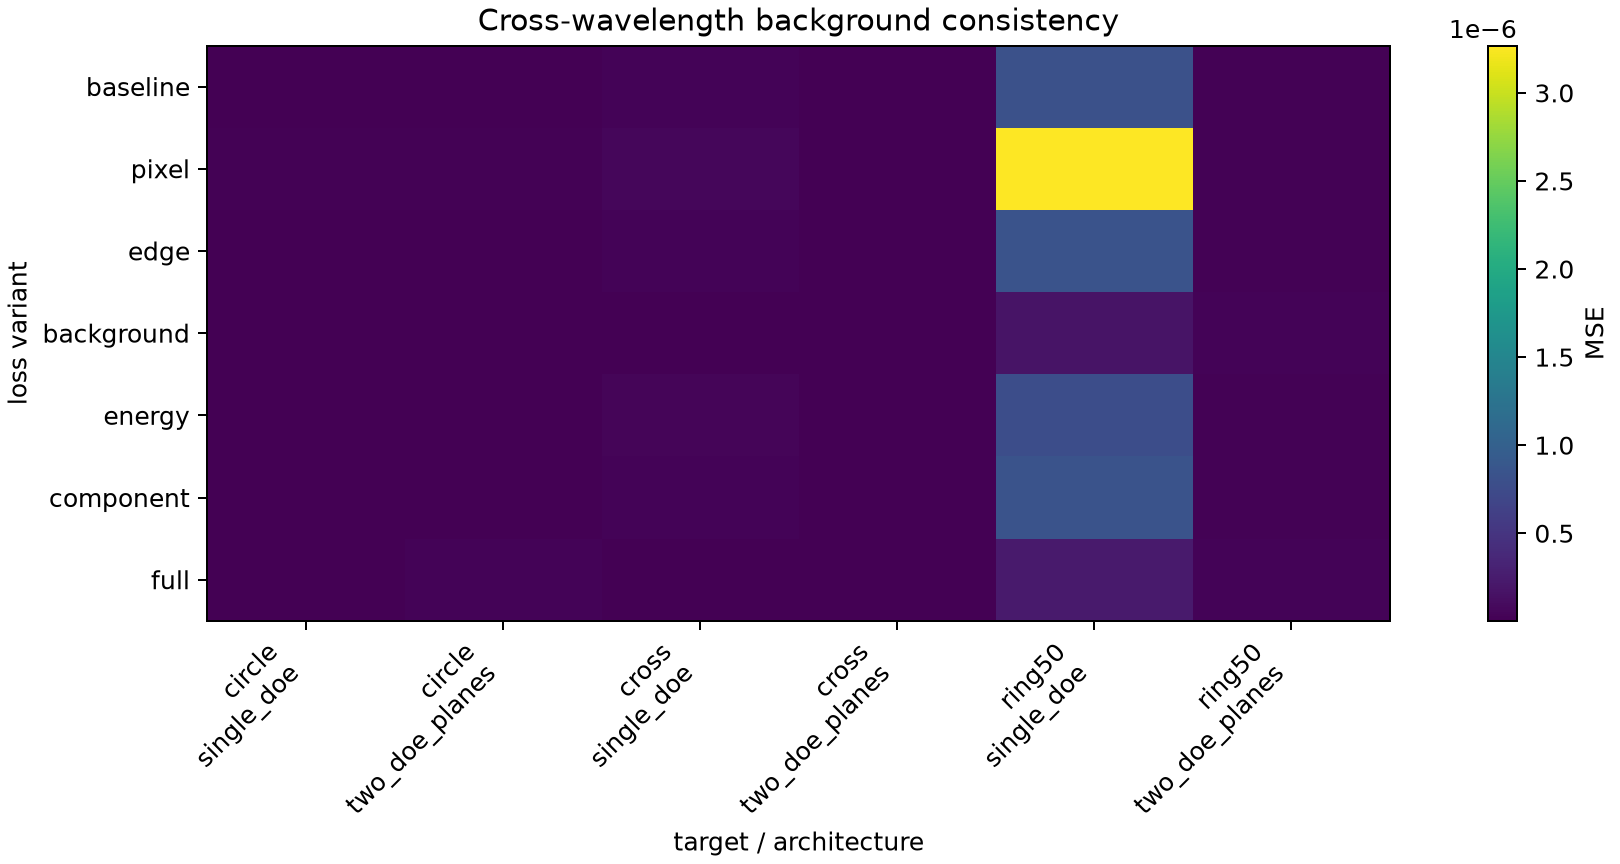
\includegraphics[width=\linewidth]{decolorization_background_heatmap.png}
  \caption{背景一致性。}
\end{subfigure}
\caption{RGB 消色散消融的主要指标热图。像素相似度、能量 CV 和质心漂移均明显改善，但背景代价不能被忽略。}
\label{fig:decolorization-heatmaps}
\end{figure}

\subsection{各类损失的作用}
逐项消融显示，pixel 变体是共同尺度像素相似度提升的主要来源；energy 变体最直接地降低 RGB ROI 绝对能量 CV，但单独使用时不保证像素纹理一致；edge 变体可降低部分边缘 MSE，却不能解决整体能量比例差异；background 变体主要约束背景结构，但如果没有效率项和形状项配合，容易牺牲有效信号；component 变体对左右光斑或双环组件比例有针对性作用，但对全场像素差异的作用有限。full 通过联合优化取得最强的共同尺度相似度，但也表现出背景上升和 ROI 效率下降的折衷。

\begin{figure}[H]
\centering
\begin{subfigure}{0.48\textwidth}
  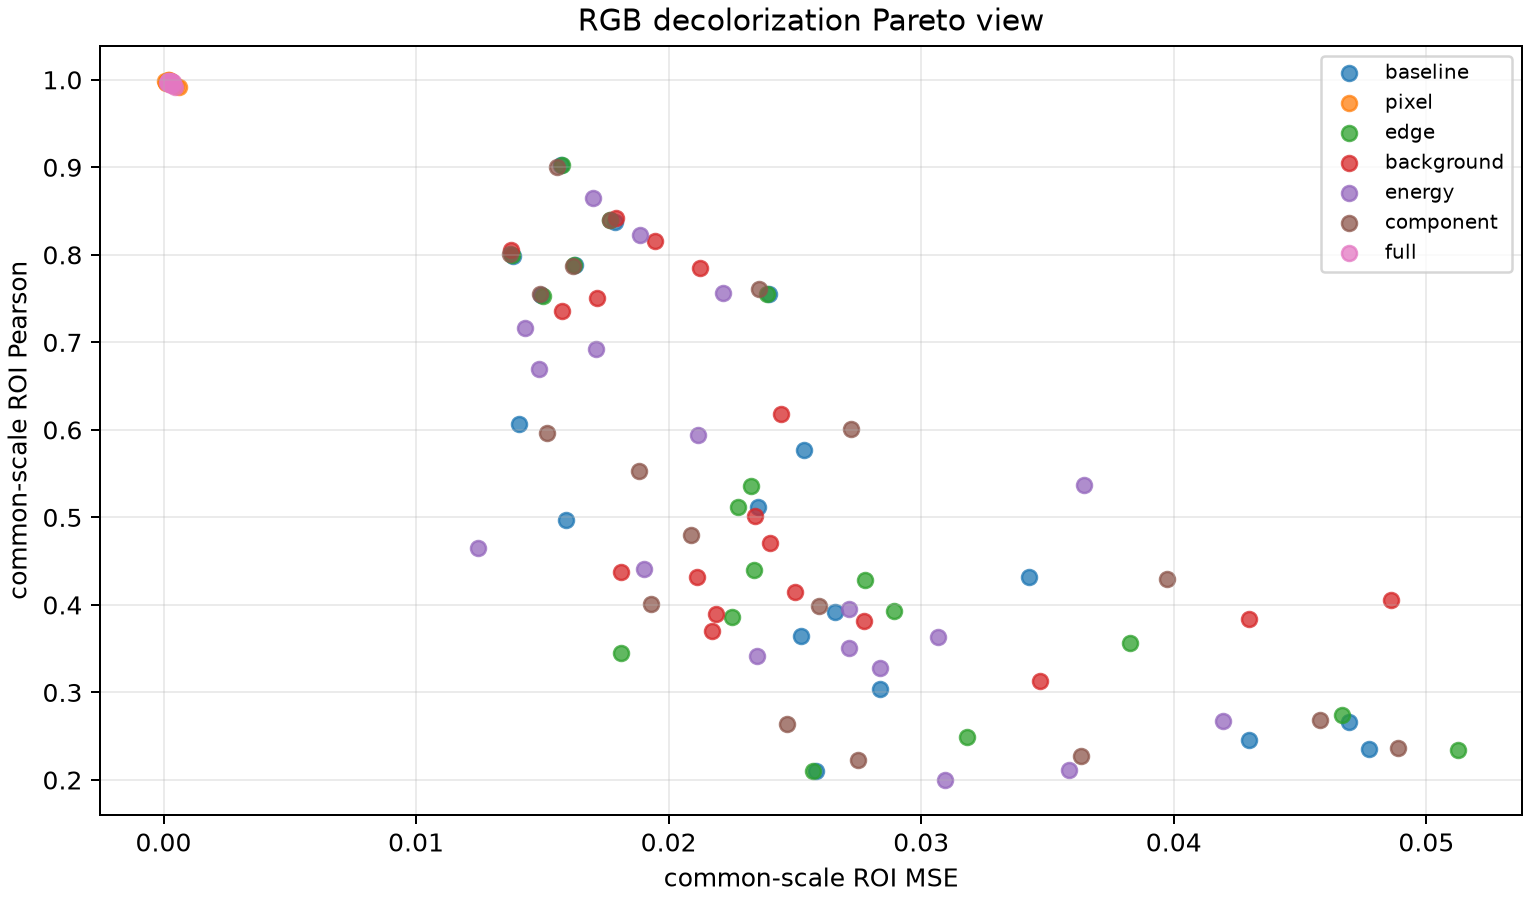
\includegraphics[width=\linewidth]{decolorization_corr_pixel.png}
  \caption{图案质量与像素一致性。}
\end{subfigure}\hfill
\begin{subfigure}{0.48\textwidth}
  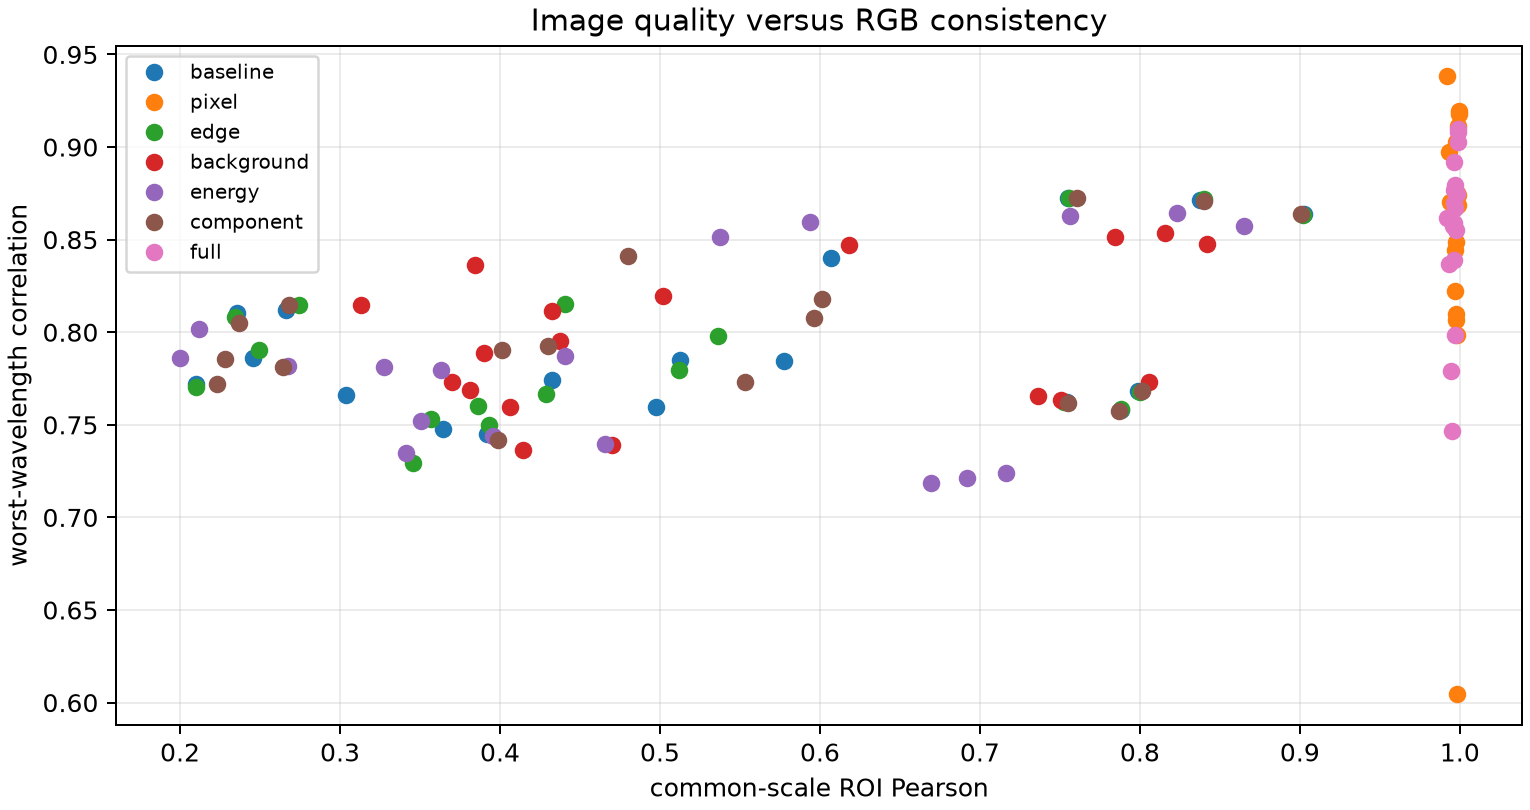
\includegraphics[width=\linewidth]{decolorization_architecture_comparison.png}
  \caption{两种光路比较。}
\end{subfigure}
\caption{消融变体和光路比较。full 的共同尺度 Pearson 接近 1，但应结合最差波长相关系数和背景一起解读。}
\label{fig:decolorization-comparison}
\end{figure}

\subsection{圆环专用指标}
在 $R=50\,\um$ 圆环中，full 单 DOE 的平均中心/环带强度比约为 $0.0245$，双 DOE 约为 $0.0078$，均低于 $0.10$ 的圆环空洞判据；平均环半径误差约为 \SI{2.5}{\micro\meter}。与 baseline 相比，单 DOE 的中心/环带比由约 $0.0170$ 增加到 $0.0245$，双 DOE 由约 $0.0006$ 增加到 $0.0078$，说明联合损失在提高 RGB 一致性的同时略微削弱了空洞对比度，但没有破坏环形拓扑。对圆环而言，后续仍应把内孔惩罚、半径一致性和背景压制作为 Pareto 约束，而不是只追求像素 Pearson。

\subsection{消色散结论}
按照预设判定规则，full 在“共同尺度 ROI Pearson 提升”“RGB 能量 CV 降低”“最差波长相关系数不显著下降”“质心漂移不增加”四项中表现良好，但在“平均背景比例增加不超过 $0.03$”这一项上整体未通过。因此最准确的结论是：
\begin{quote}
跨波长一致性损失能够显著改善当前三类目标和两种光路的 RGB 像素级空间一致性、绝对能量平衡及组件位置稳定性；但该改善在多数单元中伴随背景比例上升，因而只能称为“有限目标下的部分 RGB 消色散改进”，不能称为无代价、普适的 RGB 消色散。
\end{quote}

\section{讨论：做了什么、没有做什么}
\subsection{已经完成的工作}
本课题已经形成了从物理模型到多指标评价的完整数值链路：
\begin{itemize}
\item 建立了所有波长共享同一物理高度 $h(x,y)$ 的 DOE 相位模型；
\item 使用 S1813 两个文献折射率锚点和 Cauchy 外推完成 RGB 材料模型，并标记了 \SI{488}{nm} 的外推性质；
\item 修正了物理视场、DOE 孔径覆盖和零填充设置，完成了 $256\to512$ 粗到细流程；
\item 用角谱 FFT、角谱稠密矩阵和 Fresnel 稠密矩阵进行了小网格传播对照；
\item 完成了双波长双圆斑和双圆环研究，发现圆环的主要瓶颈是跨波长位置配准；
\item 将目标扩展到方形、十字、三角形三圆斑、实心三角形和不对称双圆斑，并完成 RGB 泛化比较；
\item 比较了单 DOE、双 DOE 和历史上的薄透镜光路；
\item 重新生成了共同色标、形状归一化和绝对能量指标，避免把显示归一化误解为真实颜色一致；
\item 完成了 $126$ 次 RGB 跨波长消色散损失正式消融，保存了配置、损失历史、三色像面、高度图和汇总指标。
\end{itemize}

\subsection{明确没有完成的工作}
以下内容不应从本文的数值结果中推断出来：
\begin{itemize}
\item 没有加工实际 DOE，也没有搭建光学平台进行实验测量；
\item 没有使用实测的 S1813 完整可见光色散曲线；
\item 没有把偏振、吸收、反射、表面粗糙度、材料非均匀性和全波电磁效应纳入模型；
\item 没有把高度量化、最小特征尺寸和制造误差作为本阶段主实验；
\item 没有对整个连续可见光谱进行训练，只做了离散 RGB 设计点以及有限的连续波长抽样验证；
\item 没有使用真实激光功率谱、探测器响应或 CIE 色度学模型，因此 RGB 合成图不能直接解释为人眼真实颜色；
\item MRAF 仍是 Adam 中的背景混合/偏置风格项，不是独立实现的经典 MRAF/GS 投影算法；
\item \texttt{doe\_fourier\_lens} 已经被验证，但由于共同色标下色散明显，未进入 RGB 消色散主结论；
\item 结果不支持“任意目标图案均可由共享高度 DOE 稳定消色散”的结论。
\end{itemize}
这些限制并不否定本研究的价值，而是界定了结论的适用范围。当前工作的主要贡献在于把“看起来颜色接近”拆解为可检验的传播、空间、能量和背景指标，并通过正式消融显示不同损失项究竟改善了什么、又牺牲了什么。

\section{结论与下一步}
\subsection{主要结论}
本研究得到以下结论：
\begin{enumerate}
\item 角谱 FFT 实现、居中坐标和零填充约定经过小网格稠密矩阵验证，角谱稠密矩阵与 FFT 的相对 L2 误差低于 $1.65\times10^{-7}$；传播能量误差处于 $10^{-7}$ 量级。Fresnel 核与角谱传播存在有限采样和近似模型差异，不能无条件互换。
\item 双波长共享高度 DOE 能形成清晰双圆斑和空心圆环；圆斑的跨波长位置较稳定，而圆环的主要困难是环带和环中心的横向配准。
\item RGB 多图案实验说明十字和较大圆环相对容易重建，$R=50\,\um$ 圆环、双圆斑和尖角图案的性能更依赖采样、几何损失和背景权重。方法在有限目标上可迁移，但不具有任意图案泛化的证据。
\item RGB 跨波长 pixel/absolute-energy 一致性损失显著提高了六个目标--光路单元的共同尺度 ROI Pearson，并降低了 RGB ROI 能量 CV；full 还显著降低了组件质心漂移。
\item full 同时增加了多数单元的背景比例，因此当前消色散结果属于“像素和能量一致性明显改善，但背景代价仍未解决”的部分成功。
\item 双 DOE 在加入跨波长一致性损失后表现出很低的 RGB 质心漂移和能量 CV，但并非所有目标上都保持更低背景或更高 ROI 效率；增加光学面数不是自动消除色散的充分条件。
\end{enumerate}

\subsection{下一阶段建议}
后续工作应优先解决已经暴露出的指标冲突，而不是单纯增加迭代次数：
\begin{enumerate}
\item 对 full 损失做背景--像素一致性 Pareto 扫描，降低像素项或增加背景项的后期权重，避免通过制造背景来获得共同 Pearson；
\item 为圆环加入跨波长环半径、环中心和内孔泄漏的显式联合约束，并对环宽进行采样敏感性扫描；
\item 对方形、十字和实心三角形加入基于 signed distance 的边界损失、顶点误差和边缘粗糙度指标；
\item 在通过数值指标筛选后，再加入高度量化、最小特征尺寸、高度扰动和孔径边缘误差；
\item 用实测 S1813 色散和真实 RGB 入射功率替代当前的两点 Cauchy 外推；
\item 对双 DOE 进一步研究不同材料、不同高度上限和独立面间距是否真正改善内部纹理，而不只是改善质心；
\item 最后进行实物加工和光学平台验证，检查模拟中没有包含的偏振、吸收、反射和加工误差。
\end{enumerate}

\section*{致谢与可复现性说明}
本报告中的正式图表均来自工作目录中的结果文件，而不是 smoke test 或 pilot 结果。传播验证使用 \texttt{results/propagation\_convergence/}；双波长圆斑/圆环使用 \texttt{results/ring\_optimization/}；RGB 泛化使用 \texttt{results/rgb\_generalization\_corrected/analysis/}；共同色标评价使用 \texttt{results/rgb\_imageplane\_evaluation/}；RGB 消色散消融使用 \texttt{results/rgb\_decolorization/}。正式消融的总汇总位于 \texttt{summary.json}、\texttt{summary.csv} 和 \texttt{ablation\_summary.csv}，每个运行目录还保留 \texttt{metrics.json}、\texttt{loss\_history.json}、像面图和高度图。论文源文件为本文件，图表副本位于 \texttt{report/figures/}。

\appendix
\section{正式 RGB 消融的配置摘要}
\begin{table}[H]
\centering
\caption{正式 RGB 消融实验的复现参数。}
\label{tab:reproducibility}
\resizebox{\textwidth}{!}{%
\begin{tabular}{ll}
\toprule
项目 & 参数 \\
\midrule
波长 & 488/532/633 nm \\
输入功率 & $1:1:1$ \\
目标 & circle、cross、ring50 \\
光路 & single\_doe、two\_doe\_planes \\
损失变体 & baseline、pixel、edge、background、energy、component、full \\
随机种子 & 7、17、27 \\
粗网格 / 迭代 & $256\times256$、\SI{10}{\micro\meter}、120 次 \\
精网格 / 迭代 & $512\times512$、\SI{5}{\micro\meter}、400 次 \\
DOE 孔径半径 & \SI{1}{mm} \\
传播距离 & 单 DOE \SI{50}{mm}；双 DOE 每段 \SI{25}{mm} \\
高度上限 & \SI{1.4}{\micro\meter} \\
零填充 & $2$ \\
设备 & CUDA；NVIDIA GeForce RTX 5060 Ti \\
总运行数 & $7\times3\times2\times3=126$ \\
\bottomrule
\end{tabular}}
\end{table}

\section{报告图表的解释边界}
本文中的线性强度图保留实际通道幅度，共同 dB 图共享参考峰值，形状归一化图只用于空间结构观察。三色合成图采用 488 nm 映射蓝色、532 nm 映射绿色、633 nm 映射红色的显示约定，并明确不作 CIE 色度学渲染解释。所有百分比、相关系数和误差均来自离散采样的数值评价；例如 \SI{5}{\micro\meter} 网格下的圆环半径误差不应被解读为真实器件具有亚像素测量精度。

\begin{thebibliography}{99}
\bibitem{kim2012}
G. Kim, J. A. Domínguez-Caballero, and R. Menon, ``Design and analysis of multi-wavelength diffractive optics,'' \emph{Optics Express}, vol. 20, no. 3, pp. 2814--2823, 2012. DOI: \href{https://doi.org/10.1364/OE.20.002814}{10.1364/OE.20.002814}.

\bibitem{chen2016}
M. Chen, C. Wang, Y. Gu, and Q. Tan, ``Diffractive optical element with same diffraction pattern for multicolor light-emitting diodes,'' \emph{Applied Optics}, vol. 55, no. 1, pp. 159--165, 2016. DOI: \href{https://doi.org/10.1364/AO.55.000159}{10.1364/AO.55.000159}.

\bibitem{bowman2015}
D. Bowman, P. Ireland, G. D. Bruce, and D. Cassettari, ``Multi-wavelength holography with a single spatial light modulator for ultracold atom experiments,'' \emph{Optics Express}, vol. 23, no. 7, pp. 8365--8372, 2015. DOI: \href{https://doi.org/10.1364/OE.23.008365}{10.1364/OE.23.008365}.

\bibitem{goodman}
J. W. Goodman, \emph{Introduction to Fourier Optics}, 3rd ed., Roberts \& Company Publishers, 2005.

\bibitem{bornwolf}
M. Born and E. Wolf, \emph{Principles of Optics}, 7th ed., Cambridge University Press, 1999.
\end{thebibliography}

\end{document}
